\documentclass[a4paper,11pt]{report}
\usepackage[T1]{fontenc}
\usepackage[utf8]{inputenc}
\usepackage{lmodern}
\usepackage{graphicx}
\usepackage{listings}
\usepackage{amsmath}
\usepackage{amssymb}
\usepackage{multirow}

\title{Locus 0.8 Manual}
\date{March 28, 2022}
\author{}

\begin{document}

\maketitle 

\newpage

\tableofcontents

\newpage 

\chapter{Preliminaries}

\section{Introduction}
The idea of a topos was expounded upon by Grothendeick in his work in algebraic geometry. His idea was to consider topological spaces in algebraic geometry by reference to their topoi of sheaves. The idea of a Grothendeick topos was then generalized by Lawvere and Tierney's idea of an elementary topos. This lead to two different kinds of topos:

\begin{itemize}
 \item Elementary topoi: the topos $Sets^C$ of presheaves on a category $C$
 \item Grothendeick topoi: the topos $Sh(C)$ of sheaves on a site $C$
\end{itemize}

Another issue that has been raised in various mathematical quarters is the use of category theory in foundations. We think that amongst all the categorical frameworks proposed as a new foundation for mathematics that elementary topos theory is the most promising. The question then emerges: why do we want new foundations? \\

Set theory was an effective foundation of mathematics for a long time, and it has been responsible for the vast blossoming in mathematical thought since the late nineteenth century. So we need some reason to want to replace it. We argue that the need for new foundations emerges from the need to create a mathematical model of computation. \\ 

The old set theoretic philosophy that treats a function $f : A \to B$ as a set $\{(a,b) : f(a) = b \}$ of ordered pairs is suitable for mathematical foundations but it doesn't do justice to the computational role of a function. We need new foundations for handling reasoning about computations involving pure functions. We find that elementary topos theory provides such a model. We hope to show with Locus that topos theory makes for the ideal mathematical foundations for modeling computation.

\newpage

Computation is a physical process, and so it certainly cannot be divorced from the physical geometry of the universe it is a part of. The locality of computation appears in the use of memory locations on an individual machine, and even beyond that with network addresses. Computations are always localized to some place in space. \\

Computations move certain collections of memory locations to other memory locations, which leads to the idea of data dependencies. We define an abstract mathematical model of memory locations and data dependencies in terms of the topoi $Sets$ and $Sets^{\to}$. This leads to our topos theoretic foundations of computation. \\

The definition of a dataflow dependency requires that we consider a function $f: A \to B$ to be an object of the presheaf topos $Sets^{\to}$, so there is a common interface with objects of the topos $Sets$. This topos theoretic framework is broadly expanded so that we can consider objects as much as possible to be types of copresheaves. In turn this allows us to reason topos theoretically about as many kinds of object as possible. \\

The word topos means place in Greek. Locus means place in Latin. The Locus project is all about reasoning about the places that computations occur. We believe that geometric reasoning holds the key to the further development of computation, and topos theory provides us with the first steps towards realising that.

\newpage

\section{Copresheaf viewer}
We take the view that copresheaves (set valued functors) should be the main objects of mathematical discourse. Yet, this notion of a copresheaf might seem too forbidding still. To make this notion more accessible to students and users we present a copresheaf viewer. This takes a copresheaf and displays it as a labeled directed graph, and then it creates a JList for each label. \\
  
\noindent 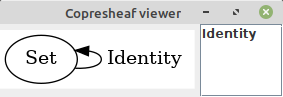
\includegraphics{{./set.png}}

Informally, a copresheaf can be seen as a kind of labeled directed graph, that has another directed graph associated to each of its labels. The copresheaf viewer actualises this informal view, to make the wide variety of copresheaves in our ontology easier to deal with. \\

\noindent 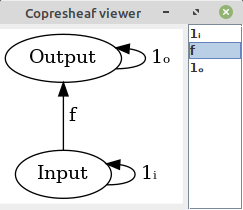
\includegraphics{{./func.png}}

The act of clicking on a label in the JList opens up a separate window containing a graphviz diagram for the function. So through the entire process, copresheaves can be seen as directed graphs layered on top of directed graphs. This only works for finite categories with finite functions defined over them, so you can't use this for say simplicial sets. But those advanced copresheaves are not used in mathematical foundations, but rather in advanced applications. For the purposes of our topos theoretic foundations, we can start with the simplest of copresheaves.

\newpage 

Displayed below is an example of a copresheaf as well as the functions associated to its labeled edges. The functions are accessed by the JList, and their JFrames are given titles that correspond to labeled edges.

\noindent 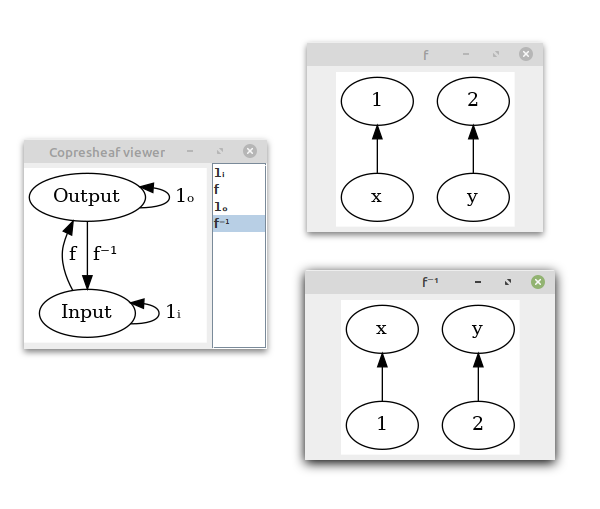
\includegraphics[scale=0.65]{{./bijection.png}}

A notable property of any copresheaf over this thin category is that $f$ and $f^{-1}$ are always going to be inverses of one another. That is realised when comparing the two different types of function diagrams displayed on the side of the copresheaf viewer. In other words, we are not interested in just any family of directed graphs layered over another directed graph but those that satisfy the axioms of a functor. \\

It is the specific satisfication of axioms that make the copresheaf formalism so powerful. For any index category $C$, the functor category $Sets^C$ always forms a topos. This provides a common topos theoretic mechanism for different kinds of copresheaves including products, coproducts, subobjects, congruences, subobject classifiers, etc. \\

The Locus system is currently a collection of techniques for dealing with computationts involving copresheaves. The copresheaf viewer is a common visual guide for all the fundamental data structures in the system.

\chapter{Topoi as foundations}

\section{Mathematical overview}
Both functional programming (formalized by $Sets^{\to}$) and logic programming (formalized by $Sets$) provide tools that can be used in topos theory. If we take these two topoi $Sets$ and $Sets^{\to}$ to be fundamental then this leads to the following trinity of concepts:


\begin{itemize}
  \item Sets: objects of $Sets$
  \item Functions: morphisms of $Sets$ and objects of $Sets^{\to}$
  \item Morphisms of functions: morphisms of $Sets^{\to}$
\end{itemize}

The fact that functions are simultaneously objects and morphisms keeps this from being a four element collection. The basic concepts of $Sets$ are familiar from classical set theory. The topos $Sets^{\to}$ on the other hand, is the arrow category of $Sets$. Let $f : A \to B$ be a function, then $(I,O)$ is a subalgebra of $f$ provided that 

\[ \forall i \in I : f(i) \in B \]

On the other hand let $(P,Q)$ be a pair of equivalence relations. Then $(P,Q)$ is a congruence of $f$ provided that 

\[ \forall a,b : (a =_P b) \Rightarrow (f(a) =_Q f(b)) \]

In other words, whenever a pair of elements are equal with respect to $P$ then their outputs over $f$ are equal with respect to $Q$. Unlike classical congruences, these congruences of functions are defined by an ordered pair of partitions instead of a single partition. Let $f: A \to B$ be a function then if $(I,O)$ is a subalgebra $f_{(I,O)}$ is a subobject of $f$ and if $(P,Q)$ is a congruence tehn $f_{(P,Q)}$ is a quotient.

\newpage 

Suppose we have that $(a =_P b) \Rightarrow f(a) =_Q f(b)$. Then for any $C \in P$ where $C$ is an equivalence class of the relation $P$ we can define $f_{(P,Q)}(C)$ to be $\pi_Q(c)$ for any $c \in C$ such that $\pi_Q$ is the projection function associated with $Q$. This is a computable formalism for defining the quotient of a function by a congruence. \\
\\ 
Let $f: A \to B$ be a function and suppose that $S \in A$ then the minimal subobject of $f$ containing $S$ as its input set is $(S,f(S)$. On the other hand, suppose that $T \subseteq B$ then $(f^{-1}(T),T)$ is the largest subobject of $f$ that has $T$ as its output set. It follows that subobjects of functions can be defined by the image and inverse image functors.
\\ \\
We naturally dualize this by defining the partition image and inverse image of a function. Let $f : A \to B$ be a function and suppose that $P$ is a partition of $A$. Then let $F = \{f(C) : C \in P\}$ be the family of images of equivalence classes of $P$ with respect to $f$. We turn this into a relation by taking $\cup \{ S^2 : S \in F \}$ and then turn it into an equivalence relation by transitive closure. The result is the largest quotient that has $P$ as its input partition.
\\ \\
We then dualize this to the idea of a partition inverse image. The partition inverse image is computationally easier to perform because inverse images preserve disjointness. Therefore let $Q$ be a partition of $B$, then we can form the family of images $\{f(C) : C \in Q \}$ and this automatically is a valid set partition of $A$. We can then form the smallest quotien that has $Q$ as its output partition.
\\ \\ 
This demonstrates that the two operations of images and inverse images are categorically dual to one another in the topos $Sets^{\to}$. We therefore distinguish from now on between set images and inverse images on the one hand and partition images and inverse images on the other. The later concept, that of a partition inverse image is going to be useful to us when we consider data dependencies which can be mathematically modeled using congruences in the topos $Sets^{\to}$.
\\ \\
Let $f: A \to B$ be a function and suppose $(X,Y)$ is a pair of subsets of $A$ and $B$ then the subalgebraic closure of $(X,Y)$ is equal to $(X, Y \cup f(X))$. Likewise, the congruence closure of $(P,Q)$ is simply $(P, f(P) \cap Q)$. Equipped with these two dual closure operations, the subobjects and congruences of a function $f: A \to B$ form lattices which we denote $Sub(f)$ and $Con(f)$. The union and intersection of subalgebras is again a subalgebra, while the intersection of congruences is again a congruence.

\newpage 

A morphism in $Sets^{\to}$ from $f : A \to B$ to $g : C \to D$ is an ordered pair of functions $(i: A \to C,o: B \to D)$ that satisfies the following commutative diagram:

\noindent 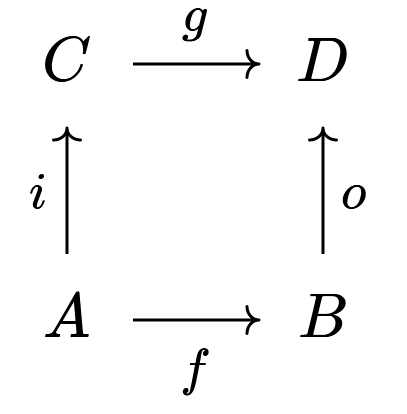
\includegraphics[scale=0.4]{{./square.png}}

This commutative diagram is again a copresheaf, so morphisms of functions can be viewed like this in the copresheaf viewer. The topos $Sets^{\to}$ has epi-mono factorisations for each morphism of functions. Congruences are equivalence classes of epimorphisms and subalgebras are congruence classes of monomorphisms, so we can say that each morphism of functions is associated to a subalgebra and a congruence. Let $(f,g)$ be a pair of functions then the subalgebra is determined by the ordered pair $(I,O)$ of images of $f$ and $g$ and the congruence is the pair $(P,Q)$ of equivalence relations $P$ and $Q$ that are the kernel of $f$ and $g$ respectively. 
\\ \\
Finally, the subobject classifier in $Sets^{\to}$ is constructed as follows. Firstly, you construct an object of truth values which is the function $\{0 \, 0, \frac{1}{2} \, 1, 1 \, 1\}$. Then given a pair $(I,O)$ defining a subobject the output set $O$ is classified by membership. On the other hand, the input set is classified in three different ways. Let $x \in A$ is $1$ provided that it is in the set $I$, it is $\frac{1}{2}$ if $f(x)$ is in $O$ and it is $0$ otherwise. Then the subobject classifier is the pair of functions $(f,g)$ to the object of truth values built by combining these two functions. \\

In additoin to sets and functions, we also provide fundamental support for the topos $Sets^2$ of pairs of sets and the topos $Sets^{K_2}$ of bijections. The topos theoretic properties of both can be determined by extending the topos of $Sets$. The topos of bijections $Sets^{K_2}$ is distinguished from $Sets$ by the fact that it is a data structure containing the data of both its forwards function and its inverse. An ordinary function the other hand, doesn't ordinally come equipped with its own inverse. \\ \\

\section{The topos of sets}
A set in elementary topos theory can be treated as a copresheaf on a space with a single object: \\

\noindent 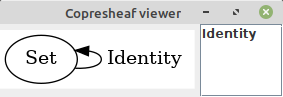
\includegraphics[scale=0.65]{{./set.png}}

Sets are implemented by a number of different data structures, and operations on these structures are handled by generic multimethods. To begin with we implement product and coproduct operations in the topos $Sets$.

\lstset {language=Lisp}
\begin{lstlisting}
(coproduct #{:a :b} #{:c :d})
;=>  #{(0 :b) (1 :d) (1 :c) (0 :a)}

(product #{:a :b} #{:c :d})
;=> #{(:a :d) (:b :d) (:a :c) (:b :c)}
\end{lstlisting}

We also have a system of predefined predicate functions that classify sets by their size:

\lstset {language=Lisp}
\begin{lstlisting}
(singular-universal? #{0})
(size-two-universal? #{0 1})
(size-three-universal? #{0 1 2})
(size-four-universal? #{0 1 2 3})
\end{lstlisting}

We use the term universal? as a special term for generalized sets in order to avoid confusion with categories (from category theory) and classes (java.lang.Class objects). The predicate set? is specialized for dealing with clojure.lang.PersistentHashSet objects. \\

A very common paradigm in computational set theory is to define separate classes for different types of sets. As an example, we define a special data type for dealing with ordinals:

\lstset {language=Lisp}
\begin{lstlisting}
(Ordinal. 5)
;=> #5
\end{lstlisting}

The universal predicate is then overwritten to designate that ordinals are universals, which means that they are like sets.

\lstset {language=Lisp}
\begin{lstlisting}
(universal? (Ordinal. 5))
\end{lstlisting}

As universal? is implemented as a multimethod you can also override it to define your own set classes. As we will see a wide variety of set abstractions are defined each with their own unique performance characteristics.

\newpage 

Every universal is a clojure.lang.IFn and so it can be called like a function to determine membership. Enumerated universals like ordinals also implement clojure.lang.Counted and clojure.lang.Seqable. This allows us to use Clojure's built in generic collection functions on seqable universals such as ordinals.

\lstset {language=Lisp}
\begin{lstlisting}
(count (Ordinal. 5))
;=> 5

(seq (Ordinal. 5))
;=> (#0 #1 #2 #3 #4)
\end{lstlisting}

In addition to implementing Clojure's built in protocols, we also provide generic versions of the functions in clojure.set. These allow us to use union and intersection operations without ever leaving the Ordinal data type:

\lstset {language=Lisp}
\begin{lstlisting}
(union (Ordinal. 4) (Ordinal. 5))
;=> #5

(intersection (Ordinal. 4) (Ordinal. 5))
;=> #4
\end{lstlisting}

Without this specification of the union and intersection operations the basic point of the Ordinals construction, which is the embedding of the total order $\omega$ and other well orders in a universe of sets, would be lost. With this we recover some of their mathematical flavour. \\

We also find it valuable to define some large sets that would otherwise take too much memory for us to define extensionally. Such seqable universals use an underlying lazy sequence combined with a predicate so that values are computed on demand.

\lstset {language=Lisp}
\begin{lstlisting}
(def million (seqable-interval 0 1000000))

(count million) 
;=> 1000000

(million 1)
;=> true

(million 1.5)
;=> false
\end{lstlisting}

In this example, we use seqable-interval to create a lazy set of the first one million integers. We demonstrate that this overloads clojure.lang.Counted so that we can easily compute the cardinality of this set. Calling the collection as a function tests for membership, it includes integers like one but not decimals and fractions which are not in the seqable interval. 

\newpage 

We also provide a difference function from elementary set theory. It overrides clojure.set/difference to work on other classes of universals.

\lstset {language=Lisp}
\begin{lstlisting}
(difference #{0 1 2 3} #{0 1})
;=> #{2 3}

(set (difference (Ordinal. 5) (Ordinal. 3)))
;=>   #{#4 #3}
\end{lstlisting}

One other function from elementary set theory is the power-set function which produces all subsets of a set:

\lstset {language=Lisp}
\begin{lstlisting}
(power-set #{0 1 2})
;=> #{#{0 1} #{} #{0 1 2} #{2} #{1} #{1 2} #{0 2} #{0}}
\end{lstlisting}

The bruteforce power-set function is not practical to use because the power set grows at an exponential rate. This is another circumstance that calls for the definition of our own set class, which we provide with PowerSet.

\lstset {language=Lisp}
\begin{lstlisting}
(PowerSet. #{0 1 2})
;=> "P(#{0 1 2})"
\end{lstlisting}

Then the power set data type implements all the relevant protocols and it overrides the intersection multimethod:

\lstset {language=Lisp}
\begin{lstlisting}
(count (PowerSet. #{0 1 2})
;=> 8

(seq (PowerSet. #{0 1 2}))
;=> #{#{0 1} #{} #{0 1 2} #{2} #{1} #{1 2} #{0 2} #{0}}

(universal? (PowerSet. #{0 1 2}))
;=> true

((PowerSet. #{0 1 2}) #{0 1})
;=> true

((PowerSet. #{0 1 2}) #{3 4})
;=> false

(intersection (PowerSet. #{0 1 2}) (PowerSet. #{1 2 3}))
;=> P(#{1 2})
\end{lstlisting}

The PowerSet class is a member of the universal? predicate because it is a type of generalized set. It is a generalized set that implements clojure.lang.Seqable and clojure.lang.Counted, but there are other types of universals that do not and these are provided by the Universal class. The Universal class simply wraps a predicate function to tag it as a universal. It then operates like any other clojure.lang.IFn. 
\newpage 

Here is an example of a universal that defines the set of perfect numbers amongst the positive integers:

\lstset {language=Lisp}
\begin{lstlisting}
(def perfect-number? 
  (Universal. 
    (fn [n] 
      (and 
        (positive-integer? n)
        (= (* 2 n) (apply + (divisors n)))))))
\end{lstlisting}

We can then call universal? on perfect-number? and it will return true, because the universal? multimethod looks for members of the Universal class.

\lstset {language=Lisp}
\begin{lstlisting}
(universal? perfect-number?) 
;=> true
\end{lstlisting}

Overriding the definition of a set and providing implementations aside from clojure.lang.PersistentHashSet does pose one significant issue: now we can have equal sets that are in different data types. Their equality won't then be determined by the equals method of java.lang.Object. We solve this with the equal-universals? method.

\lstset {language=Lisp}
\begin{lstlisting}
(equal-universals? (seqable-interval 0 3) #{0 1 2})
;=> true

(equal-universals? 
  (PowerSet. #{0 1}) 
  #{#{} #{0} #{1} #{0 1}})
;=> true
\end{lstlisting}

The subobjects in the topos $Sets$ are described by the power set. The dual concept is the set of all partitions of a set. 

\lstset {language=Lisp}
\begin{lstlisting}
(set-partitions #{0 1})
;=> #{#{#{0 1}} #{#{1} #{0}}}
\end{lstlisting}

The bell number function can be used to compute the number of elements in the quotient lattice of a finite set:

\lstset {language=Lisp}
\begin{lstlisting}
(bell-number 4)
;=> 15
\end{lstlisting}

The power-of-two function on the other hand computes the cardinality of the power set. Subobjects and quotients of $Sets$ are dual to one another in category theory. One last set theoretic function currently implemented is symmetric-difference. All of these functions provide us with the means to handle the topos $Sets$, but it is not always sufficient to restrict ourselves to working only with sets. Practical experience with computer algebra demonstrates that we often also need multisets.

\newpage 

The apache commons collections framework provides a Java-based implementation of mutable multisets that you can use in your applications and programs. We opt instead to create our own Clojure based implementation of multisets that uses persistent hash collections internally. Thusly, a multiset can be defined like so using its constructor:

\lstset {language=Lisp}
\begin{lstlisting}
(Multiset. {:x 10, :y 2, :z 3})
\end{lstlisting}

The multiset function automatically handles conversion of Clojure's collections such as sequences, vectors, sets, hashes, etc into multisets. So this is often a more convenient way of creating multisets then using the hash function.

\lstset {language=Lisp}
\begin{lstlisting}
(multiset '(0 0 0 1 1 2))
;=> *{0 0 0 1 1 2}

(multiset [0 0 1 1])
;=> *{0 0 1 1}
\end{lstlisting}

The support function determines the underlying set of keys of the persistent map that defines the multiset:

\lstset {language=Lisp}
\begin{lstlisting}
(support (multiset [0 0 1 1]))
;=> #{0 1}
\end{lstlisting}

The multiplicity function plays the role of getCount in the apache commons collections library.

\lstset {language=Lisp}
\begin{lstlisting}
(multiplicity (multiset '(0 0 0 1 1 2)) 0)
;=> 3
\end{lstlisting}

Let $S$ be a set, then $F(S)$ is a lattice ordered free commutative monoid of multisets with members in $S$. The monoid operation of multisets is multiset addition:

\lstset {language=Lisp}
\begin{lstlisting}
(add (multiset '(0 0 1)) (multiset '(2 2 1)))
;=> *{0 0 1 1 2 2}
\end{lstlisting}

A basic reason for introducing multisets into set theory, is so that we can embedd sets in some universe into a free commutative monoid. This allows us to add sets counting multiplicity.

\lstset {language=Lisp}
\begin{lstlisting}
(apply add #{#{0} #{0 1}})
;=> *{0 0 1}
\end{lstlisting}

The set system we just added together $\{\{0\}, \{0 \, 1\}\}$ is the set theoretic definition of the ordered pair. We can test for multisets produced this way with kurawski-pair-multiset?

\lstset {language=Lisp}
\begin{lstlisting}
(kuratowski-pair-multiset? (multiset '(0 0 1)))
;=> true
\end{lstlisting}

\newpage

The multiset-difference function removes elements from multisets counting multiplicity. It is therefore distinguished from the more basic difference function of set theory.

\lstset {language=Lisp}
\begin{lstlisting}
(multiset-difference (multiset '(0 0 0 1 1 2)) (multiset '(0 0 1)))
;=> *{0 1 2}
\end{lstlisting}

The functions join and meet handle the operations in the lattice of multisets. The functions iterate-multiset, multiset-division, and multiset-remainder handle repeated multiset addition and its inverse.

\lstset {language=Lisp}
\begin{lstlisting}
(iterate-multiset (multiset '(0 1)) 3)
;=> *{0 0 0 1 1 1}

(multiset-division (multiset '(0 0 0 1 1 1)) 3)
;=> *{0 1}

(multiset-remainder (multiset '(0 0 1 1 1)) 2)
;=> *{1}
\end{lstlisting}

At this point, we have to stop to take note of some new terminology. In the available literature, there is hardly anything on sets of multisets. Some articles have been written that deal with sets of multisets by referring to them as "macrosets." We refer to sets of multisets as clans because that is a more convenient terminology. Thusly, to get all subobjects of a multiset we suggest you use the power-clan function.

\lstset {language=Lisp}
\begin{lstlisting}
(power-clan (multiset '(0 1 1))
;=> #{*{1 1} *{0 1} *{1} *{} *{0} *{0 1 1}}
\end{lstlisting}

The seqable-power-clan function creates a lazy version of the set of all submultisets of a multiset, which only produces a sequence of its members on demand. Similar to other seqable universals previosusly described such as ordinals. One other interesting multiset function is the dist function, which yields the corresponding relative multiplicities of each element in a map structure.

\lstset {language=Lisp}
\begin{lstlisting}
(dist (Multiset. {:x 1, :y 2, :z 3}))
;=> {:y 1/3, :z 1/2, :x 1/6}
\end{lstlisting}

The individual elements of the distribution can be acquired by the relative-multiplicity function. The mark of a multiset is its multiset of relative frequencies. The multiplicities-map function restores the underlying map of the multiset. Several properties like maximum multiplicity, minimum multiplicity, repetitiveness, unequalness, order, and exponent are defined. The order is the size of the support. The exponent is the gcd of multiplicities. The repetitiveness checks how for a multiset is from being a set. The number-of-multiset-parts function determines the cardinality of the power clan.

\newpage 

Finite elements of the topos $Sets$ are classified by reference to their cardinalities. We have a number of of pre defined subsets of $\mathbb{N}$, which can be used to define further classes of sets by their cardinality.

\lstset {language=Lisp}
\begin{lstlisting}
(def prime-sized-universal?
  (Universal. 
    (fn [coll] 
      (and 
        (seqable-universal? coll)
        (prime-number? (count coll))))))
\end{lstlisting}

The corresponding notion for multisets is that of an additive partition. Every finite multiset is associated to an additive partition by the signature function.

\lstset {language=Lisp}
\begin{lstlisting}
(signature (multiset '(0 0 1 1 2 3)))
;=> *{1 1 2 2}
\end{lstlisting}

There are several built in functions to classify multisets by their signatures, such as regular-multiset? which tests that all multiplicities of members of the multiset are equal.

\lstset {language=Lisp}
\begin{lstlisting}
(regular-multiset? (multiset '(0 0 1 1)))
;=> true
\end{lstlisting}

Sets and multisets form distributive lattices, and so do additive partitions by Young's lattice $\mathbb{Y}$. We implement the fundamental operations of $\mathbb{Y}$ using the dual functions young-join and young-meet.

\lstset {language=Lisp}
\begin{lstlisting}
(young-join (multiset '(1 1 1 1)) (multiset '(2 2)))
;=> *{1 1 2 2}

(young-meet (multiset '(1 1 1 1)) (multiset '(2 2)))
;=> *{1 1}
\end{lstlisting}

The conjugate-partition function defines the unique automorphism of $\mathbb{Y}$.

\lstset {language=Lisp}
\begin{lstlisting}
(conjugate-partition (multiset '(1 1 1 1)))
;=> *{4}

(conjugate-partition (multiset '(2 2)))
;=> *{2 2}
\end{lstlisting}

Finally, we can test for membership in $\mathbb{Y}$ using the additive-partition? function. A special case is an additive-division? which is an additive partition of a number into all equal parts. So for a number $n$ the number of additive divisors of $n$ is equal to $d(n)$, which is also the number-of-multiset-parts of its factors multiset. In order to get all partitions of a multiset use all-partitions and to get partitions into only a set number of elements use restricted-partitions.

\newpage 

At this point, we are ready to introduce what might be an original innovation of this project. Let $\mathbb{Z}_+$ be the positive integers, then the prime signature is a map to $\mathbb{Y}$.

\[ s : \mathbb{Z}_+ \to \mathbb{Y} \]

The kernel of $s$ is a partition of $\mathbb{Z}_+$ which does not form a congruence of $(\mathbb{Z}_+,*)$. We therefore cannot form a quotient binary operation, so we get around this by instead forming a quotient hypermonoid $\frac{\mathbb{Z}_+}{s}$. This takes two additive partitions and it produces the set of all possible signatures of products of numbers with the given signatures. This leads to a morphism in the category of ternary relations:

\[ s : (\mathbb{Z}_+,*) \to (\mathbb{Y},*) \]

The new operation we introduced here we call \textit{ young multiplication}. This turns the fundamental Young's lattice into a hyperalgebraic structure. Young's multiplication is hyperextensive with respect to Young's lattice, in the sense that any product of any pair of signatures is larger then both of them. \\ 

We provide a novel and new implementation of Young's multplications based upon multiset couplings. Let $a$ and $b$ be two positive integers, then their factorisations together form a binary multirelation with one another. The computation of the hyperproduct of additive partitions is then reduced to the problem of finding all multiset couplings of a pair of multisets.

\lstset {language=Lisp}
\begin{lstlisting}
(multiply-partitions (multiset '(1 2)) (multiset '(1 2)))
;=>  #{*{3 3} *{2 2 2} *{1 2 3} *{1 1 2 2} *{4 1 1} *{4 2}}

(multiply-partitions (multiset '(2 1)) (multiset '(2)))
;=>  #{*{4 1} *{2 3} *{1 2 2}}
\end{lstlisting}

Just as $(\mathbb{Z}_,+)$ is associated with a division operation, in which any factor of a number can be divided by another there is also a division hyperoperation on Young's lattice $\mathbb{Y}$. This produces for a given pair of additive partitions $p$, $q$ such that $p \subseteq q$ in $\mathbb{Y}$ the set of all partitions $x$ such that $q \in px$.

\lstset {language=Lisp}
\begin{lstlisting}
(divide-partitions (multiset '(1 2 3)) (multiset '(1 2)))
;=>  #{*{2 1} *{3} *{1 1 1}}
\end{lstlisting}

We find that our original and independent invention of Young's multiplication, helps to illuminate the basic properties of the positive integers. The multiplication of the positive integers is generalized over Young's multiplication. Together with the well known Young's lattice operations, this defines the ordered hyperalgebraic structure of additive partitions. This hyperalgebraic structure will be the subject of further research.

\section{The topos of functions}
A function  is a copresheaf on the ordered pair category which is depicted in the copresheaf viewer as below: \\

\noindent 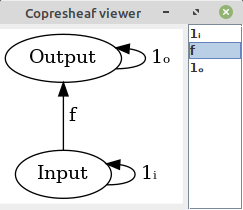
\includegraphics[scale=0.65]{{./func.png}}

A set function $f: I \to O$ is created by an ordered triple $(I,O,f)$ which can be passed into the SetFunction constructor. 

\lstset {language=Lisp}
\begin{lstlisting}
(SetFunction. #{0 1} #{2 3} {0 2, 1 3}) 

(SetFunction. #{:x :y :z} #{0 1 2 3 4 5 6} {:x 0, :y 1, :z 2}) 

(SetFunction. 
  (seqable-interval 0 10) 
  (seqable-interval 0 10)
  (fn [n] (mod (inc n) 10)))
\end{lstlisting}

Functions are simultaneously objects of $Sets^{\to}$ and the morphisms of $Sets$. Therefore, we can compose functions in the topos $Sets$.

\lstset {language=Lisp}
\begin{lstlisting}
(def f (SetFunction. #{0 1} #{2 3} {0 2, 1 3}))
(def g (SetFunction. #{2 3} #{4 5} {2 4, 3 5}))
(compose g f)
\end{lstlisting}

We can define identities in the topos $Set$ from any universal.

\lstset {language=Lisp}
\begin{lstlisting}
(identity-function #{0 1 2 3})
\end{lstlisting}

Functions are objects of the topos $Sets^{\to}$ and so just like for any object of a topos we can compute products and coproducts.

\lstset {language=Lisp}
\begin{lstlisting}
(product f1 f2)
(coproduct f1 f2)
\end{lstlisting}

The coproduct is essentially the disjoint union of the two functions. The product is defined componentwise on ordered tuples, so that if $f: A \to B$ and $g : C \to D$ are functions $f \times g : A \times C \to B \times D$ takes $(f \times g)(a,b)$ to $(f(a),g(b))$. 

\newpage 

The classical notion of a set image is dualized by partition images. These dual concepts are well defined and implemented as depicted below.

\lstset {language=Lisp}
\begin{lstlisting}
(def g (SetFunction. #{0 1 2 3} #{3 4} {0 3, 1 3, 2 4, 3 4} ))

; the set image is familiar from classical set theory
(set-image g #{0 1})
;=> #{3}

; elements in each class here are equalized by g so it
;  produces the trivial partition
(partition-image g #{#{0 1} #{2 3}})
;=> #{#{3} #{4}}

; elements in each of these classes produce different values
; so this equalizes the codomain 
(partition-image g #{#{0 2} #{1 3}})
\end{lstlisting}

Here is another example that computes for us the set inverse images and partition inverse images of a function.

\lstset {language=Lisp}
\begin{lstlisting}
(def g
  (SetFunction. 
    (seqable-interval 0 8) 
    (seqable-interval 0 4) 
    (fn [n] (int (/ n 2)))))

; the set inverse image is produce classically
(set-inverse-image g #{0 1})
;=> #{0 1 2 3}

; the partition inverse image is determined by reflection in the topos 
; of functions
(partition-inverse-image g #{#{0 1} #{2 3}})
;=> #{#{7 6 3 2} #{0 1 4 5}}
\end{lstlisting}

In addition to the dual concepts of set and partition images and inverse images, there is also a duality between function kernels and images which determine epi-mono factorisations in $Sets$.

\lstset {language=Lisp}
\begin{lstlisting}
(def func (SetFunction. #{:a :b :c :d} #{1 2 3} #{:a 1 :b 1 :c 1 :d 2}))

(function-kernel func)
;=> #{#{:a :b :c} #{:d}}

(function-image func)
;=> #{1 2}
\end{lstlisting}

\newpage 

It is often useful to get a multiset of outputs of a function instead of its images. This allows us to relate functions back to the fundamental concept of multisets we introduced earlier.

\lstset {language=Lisp}
\begin{lstlisting}
(output-multiset (mapfn {0 1, 1 1, 2 1, 3 2}))
;=> *{1,1,1,2}
\end{lstlisting}

Let $f: A \to B$ be a function, then we can classify the effect of $f$ on the input $A$ up to output isomorphism by its kernel.  We would like to use the output multiset to classify the effect of $f$ on the output $B$ up to input isomorphism. As it turns out this only works if $f$ is surjective. In the general context, we can use function selection.

\lstset {language=Lisp}
\begin{lstlisting}
(function-selection (mapfn {0 1, 1 1, 2 1, 3 2}))
\end{lstlisting}

The multiplicities of the output multiset of a function are called fiber cardinalities. It follows that the function selection is simply a map from output elements to their fiber cardinalities.

\lstset {language=Lisp}
\begin{lstlisting}
(fiber-cardinality func x)
; outputs the number of elements that output x

(fiber-cardinalities func)
; outputs all fiber cardinalities of the function
\end{lstlisting}

The predicate subfunction? tests for subalgebras of functions and io-relation? tests for congruences. Given pairs that satisfy either of these conditions we can produce subobjects and quotients with subfunction and quotient-function respectively.

\lstset {language=Lisp}
\begin{lstlisting}
(subfunction func new-input new-output)

(quotient-function func partition1 partition2)
\end{lstlisting}

These define the subobjects and quotients of a function $f$. Utilizing these concepts of the topos of functions $Sets^{\to}$ we have defined the injective quotient, the surjective subobject, and the bijective subquotient of a function.

\lstset {language=Lisp}
\begin{lstlisting}
(injective-quotient func)
(surjective-subobject func)
(bijective-core func)
\end{lstlisting}

The surjective subobject is defined by restricting the codomain of a function to its image. Let $f$ be a function with kernel $K$ then $(K,\top)$ is always a congruence of $f$ in the topos $Sets^{\to}$ so every function is associated to an injective quotient, by reducing all equivalence classes in the kernel to single elements. Then by combining both notions together we can get a bijective subquotient of any function in the topos $Sets^{\to}$.

\newpage 

A fascinating facet of the topos $Sets^{\to}$ is that it allows us to compute subobject and quotient lattices of functions. These are produced by the multimethods sub and con.


\lstset {language=Lisp}
\begin{lstlisting}
(def f (mapfn {:x 1, :y 1, :z 2}))

(sub f)
\end{lstlisting}

\noindent 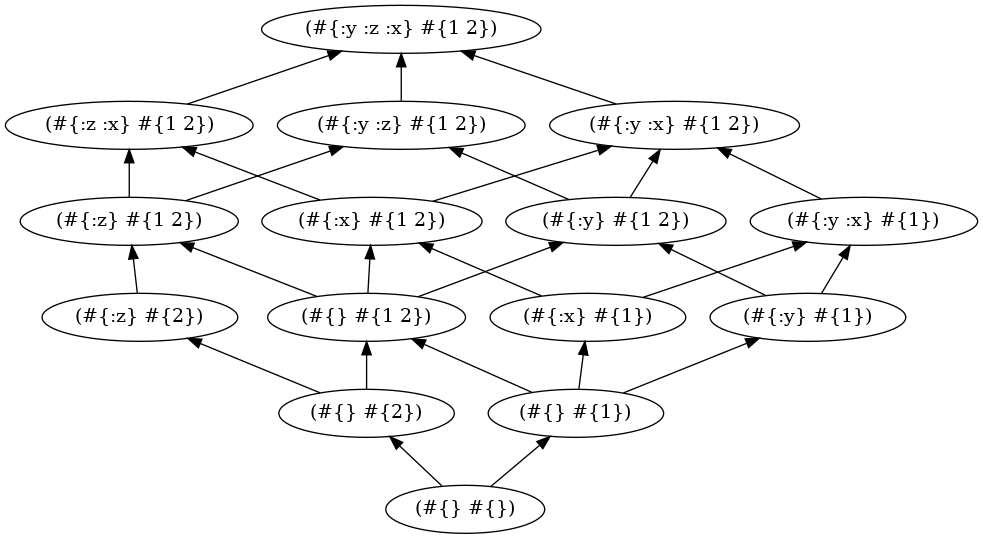
\includegraphics[scale=0.3]{{./sub.png}}

\lstset {language=Lisp}
\begin{lstlisting}
(con f)
\end{lstlisting}

\noindent 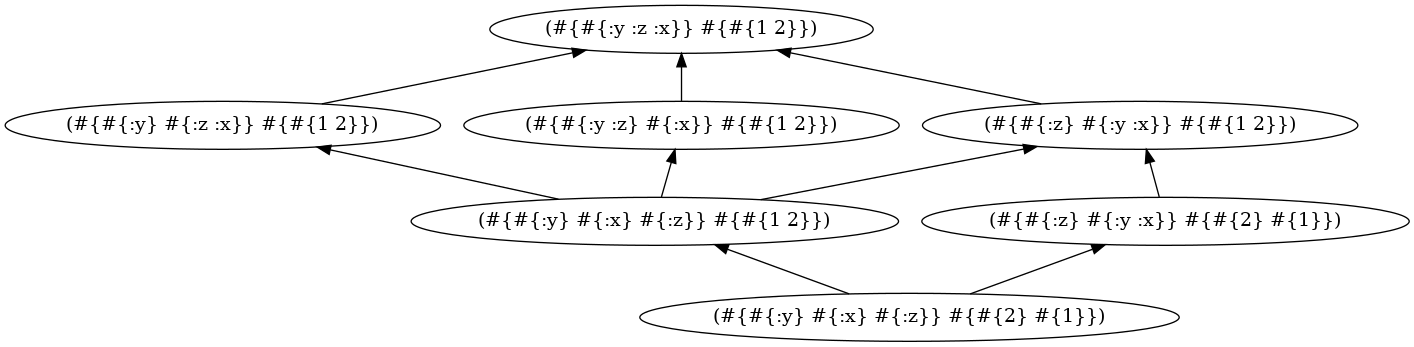
\includegraphics[scale=0.3]{{./con.png}}

At this point we can comment on the utility of the topos theoretic perspective. If we said that $f$ was a set, then $Sub(f)$ would simply be an ordinary boolean algebra and $Con(f)$ would always just be a partition lattice. By switching over to the topos $Sets^{\to}$ we get special notions of subobjects and congruences particular to functions. \\

The subobject lattice of any topos object is always distributive. In this case, the operations in the distributive lattice of subobjects of a function can be defined by componentwise union and intersection. In the congruence lattice, the meet can be defined by componentwise intersection. On the other hand, the join of two function congruences is determined by the componentwise join of the two partitions plus the function congruence closure computed by the partition image. These operations together make up our implementation of the congruence lattices of individual functions.

\newpage 

In topos theoretic foundations we start with the following basic trinity of concepts: sets, functions, and morphisms of functions. We described the first two already. The later is implemented by the MorphismOfFunctions class. A morphism of functions can be defined by a quadruple $(f,g,i,o)$ of a source function, a target function, an input map, and an output map such that these four functions make up a commutative square diagram. These outputs can be inputed into the MorphismOfFunctions constructor to create a morphism of functions instance.

\lstset {language=Lisp}
\begin{lstlisting}
(MorphismOfFunctions. f g i o)
\end{lstlisting}

The compose function is overloaded to handle either functions or morphisms of functions, depending upon the data types of its arguments.

\lstset {language=Lisp}
\begin{lstlisting}
; this composes the morphisms of functions m and n
(compose m n) 
\end{lstlisting}

$Sets^{\to}$ is also a category with identities for each of its objects, so the identity-morphism multimethod is overloaded to create the identity morphisms in $Sets^{\to}$ for function arguments.

\lstset {language=Lisp}
\begin{lstlisting}
; create in object in the topos of functions
(def func (SetFunction. #{0 1} #{2 3} {0 2, 1 3}))

; this is an identity morphism of functions
(identity-morphism func)
\end{lstlisting}

Every morphism in the topos $Sets$ has an epi-mono factorisation determined by function-kernel and function-image. Dual to this, all morphisms in the topos $Sets^{\to}$ have a function congruence and a function subobject associated to them in the lattices of subalgebras and congruences of functions.

\lstset {language=Lisp}
\begin{lstlisting}
(def m
  (MorphismOfFunctions. 
    (mapfn {:a 0, :b 1, :c 2, :d 3})
    (mapfn {:x 1, :y 2})
    (mapfn {:a :x, :b :x, :c :y, :d :y})
    (mapfn {0 1, 1 1, 2 2, 3 2})))
    
; produce the subobject associated to m
(subalgebra-component m)

; get the congruence associated to m
(congruence-component m)
\end{lstlisting}

The epi-mono factorisation in the topos of functions that this determines generalizes the basic theorems of abstract algebra, like the fundamental theorem of semigroup theory to the level of individual functions.

\newpage 

At this point, it is worth mentioning our construction of subobject classifiers in the topos $Sets$ and $Sets^{\to}$. In $Sets$ the subset-character function produces the subobject classifier.

\lstset {language=Lisp}
\begin{lstlisting}
; get a subobject classifier in the topos of sets
(subset-classifier #{0 1 2} #{0 1 2 3 4 5})

; this produces the same result as
(mapfn {0 true, 1 true, 2 true, 3 false, 4 false, 5 false})
\end{lstlisting}

In $Sets^{\to}$ this is instead handled by reference to the subfunction-character method. This produces the resulting morphism of functions that classifies truth values in the topos $Sets^{\to}$.

\lstset {language=Lisp}
\begin{lstlisting}
; construct an object in the topos of functions
(def func 
  (SetFunction.
    #{0 1 2 3}
    #{0 1 2 3 4 5 6 7}
    #{0 0, 1 2, 2 4, 3 6}))
    
; compute a subobject classifier
(subfunction-character func #{0 1} #{0 2 4})    
\end{lstlisting}

The input function of the subobject classifier is the most interesting, as the output function is simply based upon the classifier in the topos $Sets$. In this case, the subobject classifier takes 0 to 1, 1 to 1, 2 to 1/2, and 3 to 0. Two goes to 1/2 because even though it isn't in the input set, its image is in the output set. The subobject classifier completes our basic overview of the functionality provided for dealing with the topos $Sets^{\to}$. \\

We also have an ontology of morphisms of functions, as well as their properties. The classical ontology consists of a partially ordered system of predicates that classify morphisms of functions: like morphism-of-functions?, epimorphism-of-functions?, monomorphism-of-functions?, and epimorphism-of-functions?.

\lstset {language=Lisp}
\begin{lstlisting}
; test if morphism is a morphism of functions
(morphism-of-functions? morphism)
\end{lstlisting}

The identity-morphism-of-functions? predicate tests if a morphism of functions is an identity. On the other hand, input-action-morphism? tests if the output function is the identity and output-action-morphism? tests if the input function is the identity. There is a natural map from the slice categories $Sets/x$ and $x/Sets$ for any set $x$ to morphisms of $Sets^{\to}$ that relates morphisms in the slice category to input and output action morphisms.

\newpage 

\section{The topos of pairs of sets}
$Sets^2$ is the topos of copresheaves on the two object discrete category. Its objects appear in the copresheaf viewer as depicted below: \\

\noindent 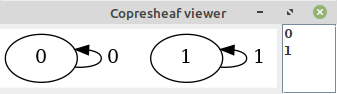
\includegraphics[scale=0.65]{{./diset.png}}

In order to create an object in the topos $Sets^2$ we use the constructor of the Diset class:

\lstset {language=Lisp}
\begin{lstlisting}
(Diset. #{:x :y} #{1/2 2/3})
;=> *(#{:x :y} #{1/2 2/3})

(Diset. #{0 1 2} #{3 4 5})
;=> *(#{0 1 2} #{4 3 5})
\end{lstlisting}

The diagram of $Sets^{\to}$ is strictly larger then $Sets^2$. Whenever you see a copresheaf over an index diagram and you want to reduce the number of morphisms in it, this produces a functor of topoi. In this case, there is a functor $f: Sets^{\to} \to Sets^2$ implemented by diset.

\lstset {language=Lisp}
\begin{lstlisting}
(let [func (SetFunction. #{0 1} #{2 3} {0 2, 1 3})]
  (diset func))
;=> *(#{0 1} #{3 2})
\end{lstlisting}

By the same token, there are two functors of topoi: $f: Sets^2 \to Sets$ and $s: Sets^2 \to Sets$ defined by further reducing an object in $Sets^2$ to either of its sets.

\lstset {language=Lisp}
\begin{lstlisting}
(def pair (Diset. #{0 1 2} #{3 4 5}))

(first-set pair)
;=> #{0 1 2}

(second-set pair)
;=> #{3 4 5}
\end{lstlisting}

It should go without saying that common functions like products, coproducts, subalgebra lattices, and congruence lattices are overloaded to deal with disets. The subalgebra lattice in $Sets^2$ is boolean, and the congruence lattice is the product of congruence lattices of $Sets$. The functions subdiset and diset-quotient are provided to get subobjects and quotients in $Sets^2$. Additional utility functions include join-disets and meet-disets which define componentwise union and intersection which turn objects in $Sets^2$ into a lattice. 

\newpage 

An ontology of disets is provided starting with the diset? function, which tests for membership in $Sets^2$.

\lstset {language=Lisp}
\begin{lstlisting}
; each of these return true
(diset? (Diset. #{0 1 2} #{3 4 5}))
(equal-diset? (Diset. #{0 1 2} #{0 1 2}))
(disjoint-diset? (Diset. #{0 1 2} #{3 4 5}))
(inclusion-diset? (Diset. #{0 1 2} #{0 1 2 3 4 5}))
(restriction-diset? (Diset. #{0 1 2 3 4 5} #{0 1 2}))
\end{lstlisting}

A morphism in the topos $Sets^2$ is simply provided by an ordered pair of functions and it is implemented in the class Difunction. The generic operations source-object and target-object are overloaded to return $Sets^2$ objects.

\lstset {language=Lisp}
\begin{lstlisting}
(def difunc
  (Difunction.
    (mapfn {:x 0, :y 1})
    (mapfn {:a -1, :b -2})))
    
(source-object difunc)
;=> *(#{:x :y} #{:a :b})

(target-object difunc)
;=> *(#{0 1} #{-1 -2})
\end{lstlisting}

The functor $f : Sets^{\to} \to Sets^2$ has a morphism part, which associates to any morphism of functions a pair of functions.

\lstset {language=Lisp}
\begin{lstlisting}
; create a morphism of functions
(def morphism (identity-morphism (mapfn {:x 1, :y 2})))

; turn the morphism of functions into a morphism of disets
(difunction morphism)
\end{lstlisting}

Finally, the topos $Sets^2$ has a subobject classifier which associates to any pair of subsets, their pair of characteristic functions. This is again defined by doubling up constructions in the topos $Sets$. The truth value in $Sets^2$ has four values, so that $Sets^2$ is considered to be a first example of a boolean topos that is not bivalent. Membership of morphisms in the topos $Sets^2$ is tested by the difunction? predicate.

\lstset {language=Lisp}
\begin{lstlisting}
(difunction? difunc)
;=> true
\end{lstlisting}

Finally, the functions function-kernel-pair and function-image-pair handle epi-mono factorisations in the topos $Sets^2$. Again they are both defined by doubling up constructions in $Sets$. They relate morphisms in $Sets^2$ to subobjects and quotient lattices.

\newpage

\section{The topos of bijections}
A bijection is a copresheaf over the index category $K_2$ consisting of two objects and two morphisms between them. This is depicted in the copresheaf viewer diagram depicted below:
 
\noindent 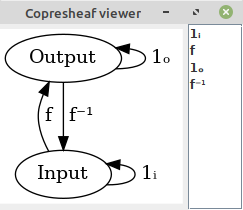
\includegraphics[scale=0.65]{{./bn.png}}

Unlike in the case of $Sets^{\to}$ the copresheaves in $Sets^{K_2}$ have different functions associated to their arrows. As it turns out these two functions $f$ and $f^{-1}$ are always inverses of one another, which make these objects into dual pairs of isomorphisms in the topos $Sets$. The Bijection constructor takes four arguments: an input, an output, a forwards function, and a backwards function.

\lstset {language=Lisp}
\begin{lstlisting}
(def invertible-increment 
  (Bijection.
    (Universal. integer?) 
    (Universal. integer?)
    (fn [n] 
      (+ n 1))
    (fn [n] 
      (- n 1))))
\end{lstlisting}

The Bijection class of course implements clojure.lang.IFn so that you can call bijections as you would any function, but more then that it implements the Invertible protocol which means that you can take any bijection and gets its inverse.

\lstset {language=Lisp}
\begin{lstlisting}
(invertible-increment 10)
;=> 11

((inv invertible-increment) 11)
;=> 10
\end{lstlisting}

Bijections are treated like the morphisms in the wide subcategory of $Sets$ of isomorphisms, so they overload the compose function. If we have two bijections $(f,f^{-1})$ and $(g,g^{-1})$ then the composition is $(g \circ f, f^{-1} \circ g^{-1})$ so that composition of inverses is backwards. 

\newpage 

There is an obvious morphism of $Sets^{K_2}$ to $Sets^{\to}$, which we provide by the underlying-function method.

\lstset {language=Lisp}
\begin{lstlisting}
; define a bijection
(def bn (mapbn {:x 1, :y 2}))

; get its underlying function
(underlying-function bn)
\end{lstlisting}

Products and coproducts are overloaded to work with any topos object rather it is a set, function, diset, or bijection.

\lstset {language=Lisp}
\begin{lstlisting}
; products and coproducts in the topos of bijections
(product bijection1 bijection2)
(coproduct bijection1 bijection2)
\end{lstlisting}

Bijections differ from functions on the level of implementation. A computable function might be invertible but without any algorithm for reversible computations. But bijections differ beyond that because they are objects of a different topos. There is an equivalence of categories between the trivial category $K_1$ and the category $K_2$. So that $Sets^{K_2}$ and $Sets$ are alike in almost every way. The subobject lattices of bijections are boolean and their congruence lattices are partition lattices. \\

By the functor $f : Sets^{K_2} \to Sets^{\to}$ every single bijection subalgebra or congruence is again a function subalgebra or congruence. The lattice of subalgebras and congruences of $Sets^{K_2}$ consist of all those subalgebras and congruences whose subobjects and quotients that preserve bijectiveness. By expanding to $Sets^{\to}$ you can get a larger lattice of subobjects or congruences. Lets create a morphism in $Sets^{K_2}$.

\lstset {language=Lisp}
\begin{lstlisting}
; create a morphism of bijections
(def morphism (MorphismOfBijections. f g i o))

; map a morphism of bijections to a morphism of functions
(underlying-morphism-of-functions morphism)
\end{lstlisting}

Again this is basically the same as $Sets^{\to}$ except a morphism in $Sets^{K_2}$ creates a morphism of functions not only for the forwards function but the inverse function as well. The subobject classifier is defined by doubling up the classifier of $Sets$:

\lstset {language=Lisp}
\begin{lstlisting}
(subbijection-character (mapbn {:a 1, :b 2}) #{:a} #{:c})
\end{lstlisting}

In general let $K_n$ be a complete thin groupoid. Then the topos $Sets^{K_n}$ of copresheaves is boolean and it has properties similar to that of $Sets$. The topos $Sets^{K_2}$ is just a simple case that we can use as a foundation for our later constructions of more advanced topoi.
\newpage 

\chapter{Topos theory of computation}

\section{The geometry of computation}
A computing device is a physical structure laid out geometrically in some manner in space. The physical detail of how memory is arranged in space is typically abstracted by the processor and the operating system to the best of their abilities. Some details of how memory is managed still seep into the user space, such as the dichotomy between RAM and hard drive disk storage which is why users need to save files. \\

The physical geometry of memory is typically as follows: at the lowest level there are the process registers and the cache. These are closest to the processor. Then their is RAM, followed by the internal hard disk, and then any external hard disks. Beyond that there are memory locations in other computers distributed in space around the world which are accessible by networking. All of this is to demonstrate the importance of the geometry of memory to computing technology. \\

The best means we have for thinking about geometry is provided by topos theory, which was invented by Grothendeick as part of his work in algebraic geometry. At this point, it might seem that we need to bring in all the complexities of Grothendeick topoi to create a mathematical model of computation and that might add significant complexity to our efforts, which we would prefer to avoid until necessary. As we shall see that is now possible. \\

All the most important machinery is there in the simplest elementary topoi like $Sets$ and $Sets^{\to}$, which almost anyone can understand. These basic elementary topoi create a simple and elegant foundation upon which anyone can build. The only complexity in our system then will come from the vast structures and semantic networks we create on top of our simple topos theoretic foundations.

\newpage 

\section{Memory locations and data dependencies}


Let $S$ be the state space of an abstract machine. Let $T$ be a transition function operating on $S$. Then by itself this yields the classical model of computation. We'd like to extend this limited approach by creating a mathematical model that takes into account the geometry of computation. As we shall see, elementary topos theory provides that perfectly.

\begin{itemize}
  \item Memory locations: congruences of the state space $S$
  \item Data dependencies: congruences of the transition function $T$
\end{itemize}

There are several key points about this formalism. Firstly, this abstracts away all details about representations. In fact, a memory location is any piece of data that can be extracted by a function. The memory location that a function accesses is determined by its kernel. At the same time, this lets us model data dependencies without regard for any particular details of representation. \\

Secondly, this integrates perfectly with our use of topos theoretic foundations. The only topoi we need in this model are $Sets$ and $Sets^{\to}$. This motivates our particular formalisation of foundations: we would like to model things as much as possible using the topoi $Sets$ and $Sets^{\to}$ as our main fundamental building blocks. This is the approach we take in this computer algebra system. \\

Thirdly, in the topos model of computation any set has memory locations and any function can have data dependencies. The quotient of a set by a memory location is the set of values that can occur in that memory location, and the quotient of a transition function by a dataflow dependency from $A$ to $B$ is the function describing how $A$ maps into $B$. \\

This defines the basic formalism we need, but in order to make of greater practical use we need to build a semantic network and ontology of information about memory locations and data dependencies of sets and functions and we need several utility classes like lenses, product decompositions, flow models, etc that help us build models of computational processes on top of our topos theoretic foundations.

\newpage 

\section{Abstract formalisation of lenses}
A lens is a set together with a getter function and a setter function. By defining a getter function, a lens still contains information about the representation of the information stored in a piece of memory. We need to abstract away all details about representation.
\\ \\
Definition. a lens type is an ordered pair $(P,Q)$ of set partitions of $S$ such that $\forall A \in P, B \in Q : |A \cap B| = 1$. The projection functions to $P$ and $Q$ then form the projection functions in the categorical definition of a product in the topos $Sets$.
\\ \\ 
Getters and setters can be defined from a lens type using our topos theoretic formalisation of memory locations and data dependencies.

\begin{itemize}
  \item Getter: a getter for a lens type is any function that has the partition $P$ as its kernel. In other words, the data stored by the lens type is $P$.
  \item Setter: a setter function is any transformation $f: S \to S$ such that $(P,P)$ and $(Q,Q)$ are data dependencies, and such that the quotient of $f$ by $(Q,Q)$ is the identity function on $Q$.
\end{itemize}

With this simple model, we have created an abstract formalisation of lenses that fits into our topos theoretic foundations. While the idea of set partitions can be used to model any place in memory the lens type can be used to model mutable state. We can create a lens type like so:

\lstset {language=Lisp}
\begin{lstlisting}
; here is a simple example of a lens type
(LensType. 
  #{#{0 1} #{2 3}} 
  #{#{0 2} #{1 3}})

; this is an example of a lens on a larger set
(LensType. 
 #{#{0 1} #{2 3} #{4 5} #{6 7}}
 #{#{0 2 4 6} #{1 3 5 7}})
\end{lstlisting}

 One function provided by Locus is to-transformation-monoid. With this function, we can take a lens type like this and convert it into the monoid of all transformations operating on the piece of mutable memory defined by the lens type. In the same vein, to-permutation-group converts a lens type to a permutation group. This demonstrates the integration of monoid actions and our model of local memory.

\newpage 

In addition to the LensType class there is a representational Lens, which provides a getter and a setter as well as the specific representation of the memory location. To create a Lens you call its constructor:

\lstset {language=Lisp}
\begin{lstlisting}
(def first-lens 
  (Lens. 
    size-two-seq? 
    (fn [coll]
      (first coll))
    (fn [coll x]
      (list x (second coll)))))
      
(def second-lens 
  (Lens. 
    size-two-seq? 
    (fn [coll]
      (second coll))
    (fn [coll x]
      (list (first coll) x))))
\end{lstlisting}

We can use the zap function to run a transformation on the lens.

\lstset {language=Lisp}
\begin{lstlisting}
(def pair '(0 1))

(zap first-lens pair inc)
;=> (1 1)

(zap second-lens pair dec)
;=> (0 0)
\end{lstlisting}

We can use nth-sequence lens to automatically get a lens from a sequence type referring to a slot within it at a given index. We can use binary-product-first-lens and binary-product-second-lens to get lens from specific cartesian products.

\lstset {language=Lisp}
\begin{lstlisting}
(def first-integer 
  (binary-product-first-lens integer? integer?))
  
(def second-integer 
  (binary-product-second-lens integer? integer?))
\end{lstlisting}

The general formula is defined by product-lens. This generalizes the fact that abstractly, a categorical product in the topos $Sets$ always creates a lens for each set involved in it. We can create local transformation monoids and permutation groups from a lens, and even local MSets and GSets. This allows us to integrate our model of the geometry of memory with the familiar structures of abstract algebra.

\newpage 

\section{Product decompositions and flow models}
Let $S$ be a set then $Con(S)$ is the lattice of all partitions of $S$. All memory locations, and indeed any piece of data that can be determined on $S$ by a function is now a part of this $Con(S)$ lattice, but often times we want to restrict this powerful model to something more manageable. Enter the ProductDecomposition class. This allows you to treat memory by specific sets of indexed locations. \\

A product decomposition creates a boolean algebra in the lattice $Con(S)$, which can be represented as a boolean algebra of sets. Our only task then is to create an antitone mapping from sets of terms in the boolean algebra to partitions in $Con(S)$. As an example, consider a set of sixteen bytes $(\mathbb{Z}_{256})^{16}$ then we can establish a product decomposition on it like so:

\lstset {language=Lisp}
\begin{lstlisting}
(def decomposition 
  (apply 
    cartesian-product-decomposition 
    (repeat 16 (seqable-interval 0 256)))
\end{lstlisting}

The memory locations can then be referred to more conveniently by their indices rather then by set partitions. We can now use this to get an equivalence relation from a set of keys.

\lstset {language=Lisp}
\begin{lstlisting}
; get the memory location storing #{0}
(get-equivalence-relation decomposition #{0})

; get the composite memory location storing #{0,1,2,3}
(get-equivalence-relation decomposition #{0 1 2 3})
\end{lstlisting}

Product decompositions generalize lens types, to arbitrary sets of variables. The to-product-decomposition function lets you convert a lens type into a product decomposition.

\lstset {language=Lisp}
\begin{lstlisting}
; create a lens type
(def lens-type 
  (LensType.
    #{#{0 1 2} #{3 4 5}}
    #{#{0 3} #{1 4} #{2 5}}))
    
; convert it into a product decomposition
(to-product-decomposition lens-type)
\end{lstlisting}

The main work that the ProductDecomposition class performs is that it handles the conversion of sets of variables into the lattice of partitions $Con(S)$ of a set $S$. This provides a more convenenient interface for handling memory locations. Next we need a new formalism for dealing with data dependencies. This is provided by the FlowModel class.

\newpage 

If we have a function $f : A \to B$ between two product types with decomposition indices $I$ and $J$ then the data dependencies of $f$ can be described always as pairs $(s,j)$ where $s$ is a set of indices in $I$ and $j$ is a single index in $J$. This reduces data dependencies to single indices. \\

This reduces data dependencies on functions to structures that look like a lot like morphisms in the allegory of sets and set relations. A set relation $r : A \to B$ maps values in $A$ to sets in $B$. So we represent this using a hash map of terms in $J$ mapped to sets in $I$. 

\lstset {language=Lisp}
\begin{lstlisting}
(def example-flow-model
  (FlowModel.
    #{0 1 2 3}
    #{0 1 2 3}
    {0 #{1 2}
     1 #{2 3}
     2 #{}
     3 #{0}}))
\end{lstlisting}

The topos $Sets^{\to}$ comes equipped with partition images and inverse images for any function $f : A \to B$. So what we want this to do is perform partition images and inverse images over our partitions represented as indices. This we provide with forwards-flow and inverse-flow.

\lstset {language=Lisp}
\begin{lstlisting}
; compute the partition image of #{1 2}
(forwards-flow example-flow-model #{1 2})
;=> #{0 2}

; compute the partition inverse image of #{0 1}
(inverse-flow example-flow-model #{0 1})
;=> #{1 2 3}
\end{lstlisting}

The product decompsition makes variables like 0,1,2,3, etc into generators in a congruence lattice of a set. So this flow model describes partition image and inverse images of the topos of functions $Sets^{\to}$ entirely in terms of sets of generators. Then the flow model is a generating set for a congruence sublattice in $Sets^{\to}$. We can test for membership in the generated sublattice of function congruences using the flow-congruence? predicate.

\lstset {language=Lisp}
\begin{lstlisting}
(flow-congruence? example-flow-model #{1 2 3} #{0 1})
\end{lstlisting}

In order to make this system complete, we finally need to be able to define functions equipped with flow models and product decompsitions, and we need to be able to get function quotients. This is provided by the CompositeFunction class. We see that the composition of functions maps contravariantly to flow models, which we use to find congruences of composite functions.

\newpage 

\section{Representing knowledge about computation}
Information about memory locations, data dependencies, and related notions should be integrated into a knowledge-based system. We extend the classical set theoretic approach to ontology to create a threefold system of semantic knowledge about computation.

\begin{itemize}
\item Set theoretic ontology: the classical ontology of entities, classes, and their membership relations to one another
\item Partition ontology: the ontology of properties, parts, and memory locations determined by lattices of apartness relations of sets
\item Dataflow ontology: the ontology of data dependencies of functions expressed in terms of the quotient lattices of functions
\end{itemize}

The set theoretic ontology can be formed traditionally, but the partition ontology and dataflow ontology are both contextualized to particular universals and functions. Suppose we have an ordered triple, then we might represent semantic knowledge about its parts: the first part, second part, third part, etc using the partition ontology. \\ 

We might further say that the butlast part contains the first and second parts and the rest part contains the second and third. This allows us to represent semantic knowledge about the hierarchy of properties of structures in terms of the topos $Sets$. \\ 

The set theoretic ontology and the partition ontology can both be defined largely classically using relations like generalisation and membership. In the third case, we need another data structure to represent data dependencies consisting of a hash map that maps a function in our knowledge base to a set of ordered pairs of congruences, which forms a generating set for the lattice of known congruences. The dataflow ontology is always going to be dependent upon the partition ontology for information on the congruences it is referring to. \\

As an example, suppose we have the Bijection class. Then in the partition ontology it might have !=source-object and !=target-object properties established in the knowledge base. Then we could add semantic data about the invert-bijection function that says that (!=source-object, !=target-object) and (!=target-object, !=source-object) are function congruences. We can then simply add the information of those pairs to our system of semantic knowledge about the invert-bijection function. So this is the basic approach we are going to take to representing semantic knowledge about data dependencies of functions in our knowledge-based system.

\newpage 

\chapter{Elementary topos theory}

\section{The topos of quivers}
A quiver is a copresheaf of the topos $Sets^{T_2^*}$ which appears as below in the copresheaf viewer: \\

\noindent 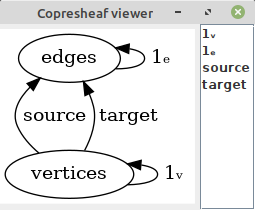
\includegraphics[scale=0.65]{{./quiver.png}}

A quiver is like a multi-directed graph. We can create a quiver either from a relation or a multirelation. In the later case, we convert the multirelation into a set of ordered pairs plus indices.

\lstset {language=Lisp}
\begin{lstlisting}
; create a quiver from a set of ordered pairs
(relational-quiver '#{(0 1) (1 2) (2 3)})

; create a quiver from a multiset of ordered pairs
(multirelational-quiver (multiset '((0 1) (1 2) (1 2) (2 3))))
\end{lstlisting}

The reverse of these are the underlying-relation and underlying-multirelation functions.

\lstset {language=Lisp}
\begin{lstlisting}
(underlying-relation quiver)
(underlying-multirelation quiver)
\end{lstlisting}

Hom classes in quivers can be computed by the quiver-hom-class function. The result is non-empty iff the argument is in the underlying-relation. \newpage

\newpage 

We demonstrated that we can use product and coproduct for sets, functions, and other elements of topoi. The same function works for quivers as they are a type of copresheaf.

\lstset {language=Lisp}
\begin{lstlisting}
; define instances of quivers
(def quiver1 
  (relational-quiver '#{(0 0) (1 1) (2 2) (0 1) (0 2) (1 2)}))
  
(def quiver2
  (relational-quiver '#{(0 0) (1 1) (2 2) (3 3) (0 1) (2 3)}))
  
; compute a product in the topos of quivers
(product quiver1 quiver2)

; compute a coproduct in the topos of quivers
(coproduct quiver1 quiver2)
\end{lstlisting}

A morphism in the topos $Sets^{T_2^*}$ can be created by the MorphismOfQuivers class in the same basic way as for a morphism of functions.

\lstset {language=Lisp}
\begin{lstlisting}
; create a morphism of quivers from q to r
(MorphismOfQuivers. q r i o)
\end{lstlisting}

Instead of a single morphism of functions, a morphism in $Sets^{T_2^*}$ now has the data of two different morphisms of functions. These can be retrieved by using morphism-of-source-functions and morphism-of-target-functions. These implement the morphic part of the dual functors $s : Sets^{T_2^*} \to Sets^{\to}$ and $t : Sets^{T_2^*} \to Sets^{\to}$. \\

The subobject classifier in the topos $Sets^{T_2^*}$ is primarily concerned with classifying the truth degree of edges in a subobject. There are now five different truth values an edge can take based upon membership of its source vertex, target vertex, and the edge itself. The subobject classifier is implemented by subquiver-character.

\lstset {language=Lisp}
\begin{lstlisting}
; create a quiver
(def quiver (relational-quiver '#{(0 1) (1 2) (2 3)}))

; get the characteristic function of a subquiver
(subquiver-character quiver '#{(2 3)} '#{1})
\end{lstlisting}

The subobject classifier in $Sets^{T_2^*}$ is just another thing which unites quivers with other topoi. Quivers also have their own subobject and quotient lattices determined by sub and con.
\newpage 

\section{Lattices and partial orders}
Lattices can be constructed out of almost anything by using the sub and con multimethods. Lets start by constructing a quiver. 

\lstset {language=Lisp}
\begin{lstlisting}
(def quiv (relational-quiver '#{(0 1) (0 2)}))
\end{lstlisting}

Then we can use the sub method to create its lattice of subobjects:

\lstset {language=Lisp}
\begin{lstlisting}
(sub quiv)
\end{lstlisting}

\noindent 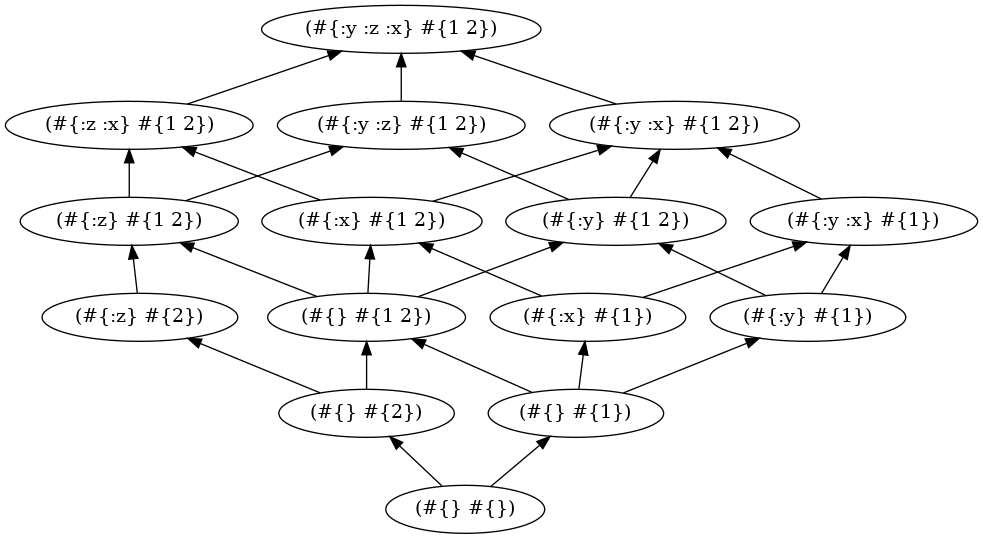
\includegraphics[scale=0.3]{{./sub.png}}

The con method can be used to create its lattice of congruences:

\lstset {language=Lisp}
\begin{lstlisting}
(con quiv)
\end{lstlisting}

\noindent 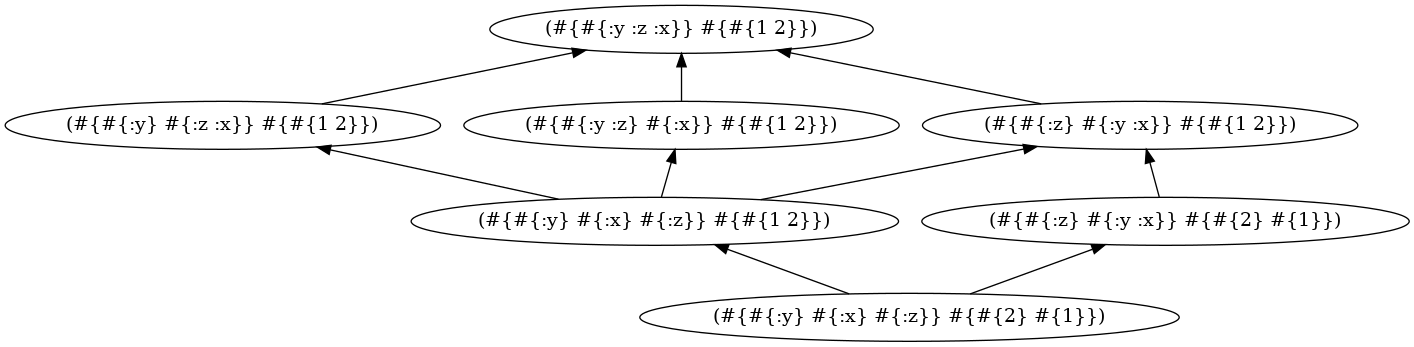
\includegraphics[scale=0.3]{{./con.png}}

The sub and con lattices can be applied to sets:

\lstset {language=Lisp}
\begin{lstlisting}
(sub #{0 1 2}) ; a boolean algebra of sets
(con #{0 1 2}) ; a geometric lattice of partitions
\end{lstlisting}

In general, subobject and congruence lattices should be computable for any object of a topos, using built in routines. The product method is overriden to handle lattices:

\lstset {language=Lisp}
\begin{lstlisting}
(product lattice1 lattice2) ; a product lattice
\end{lstlisting}

The coproduct on the other hand does not work for lattices, but the coproduct will give you a thin category $L_1 + L_2$ for any two lattices $L_1$ and $L_2$. The category of lattices is coproduct free.

\newpage 

Lattices are implemented as thin categories. This fact is confirmed by the category? and thin-category? predicates.

\lstset {language=Lisp}
\begin{lstlisting}
(category? (sub #{0 1 2}) 
;=> true

(thin-category? (sub #{0 1 2}))
;=> true
\end{lstlisting}

The elements of a lattice are objects of a category, and so we can call product and coproduct on them. The product operation is the meet and the coproduct operation is the join.

\lstset {language=Lisp}
\begin{lstlisting}
(def lattice (sub #{0 1 2 3}))
(def object1 (LatticeObject. lattice #{0 1}))
(def object2 (LatticeObject. lattice #{2 3}))

(coproduct object1 object2)
;=> #{0 1 2 3}

(product object1 object2)
;=> #{}
\end{lstlisting}

There is a forgetful functor $f: Cat \to Quiv$. It follows that every category, including lattices has an object in the topos of quivers.

\lstset {language=Lisp}
\begin{lstlisting}
(underlying-quiver lattice)
\end{lstlisting}

In order to perform computations over free lattices, we provide an abstract definition of expressions in arbitrary lattices. The coproduct operation is denoted by + and the product operation is denoted by * in the symbolic representation of lattice expressions.

\lstset {language=Lisp}
\begin{lstlisting}
(def term 
  (LatticeTerm. '(+ (* a b) (* c d))))
\end{lstlisting}

As a category $Lat$ is quite different from $Ord$. The category $Lat$ is equipped dual functors $j : Lat \to Sets^{\to}$ and $m : Lat \to Sets^{\to}$ that map lattices to their join and meet functions and lattice morphisms to their respective morphisms of functions.

\lstset {language=Lisp}
\begin{lstlisting}
; create a morphism in the category of lattices
(def morphism (LatticeMorphism. source target func))

; get the morphisms in the topos of functions
(morphism-of-join-functions morphism)
(morphism-of-meet-functions morphism)
\end{lstlisting}

Aside from lattices, the Poset class defines thin skeletal categories and MonotoneMap defines morphisms of them.

\newpage 

\section{Semigroups, monoids, and groups}
Let $(\mathbb{Z},\leq)$ be the thin totally ordered category of integers. Then the join and meet semilattices of $(\mathbb{Z},\leq)$ lack identities, and so they are semigroups and not monoids. We therefore find it necessary to implement semigroups as well as monoids, even though the former are not categories. We can create semigroups by using the semigroup-by-table function.

\lstset {language=Lisp}
\begin{lstlisting}
(def c3 
  (semigroup-by-table 
    [[0, 1, 2]
     [1, 2, 0]
     [2, 0, 1]]))
\end{lstlisting}

We can now test to see if c3 is a semigroup or a monoid:

\lstset {language=Lisp}
\begin{lstlisting}
(semigroup? c3)
;=> true

(monoid? c3)
;=> true
\end{lstlisting}

The product of semigroups is again a semigroup, but the coproduct of semigroups is a semigroupoid. 

\lstset {language=Lisp}
\begin{lstlisting}
; create a rectangular band
(product (left-zero-semigroup 2) (right-zero-semigroup 2))
\end{lstlisting}

The free-monoid method can be used to create a free semigroup on a set of generators. In addition, there is support for free bands, commutative monoids, groups, and commutative groups.

\lstset {language=Lisp}
\begin{lstlisting}
(free-monoid #{0 1 2})
\end{lstlisting}

We provide basic support for Green's relations. 

\lstset {language=Lisp}
\begin{lstlisting}
; greens preorders
(lpreorder semigroup)
(rpreorder semigroup)
(jpreorder semigroup)

; greens relations
(lrelation semigroup)
(rrelation semigroup)
(jrelation semigroup)
(drelation semigroup)
(hrelation semigroup)
\end{lstlisting}

The com method computes the computing graph of a semigroup, group, or monoid and commutativity-preorder computes the corresponding adjacency preorder of that graph. 

\newpage 

The category of semigroups can be embedded in the topos $Sets^{\to}$. This is defined by the functor $f: Sgrp \to Sets^{\to}$. The underlying-function and underlying-morphism of functions methods handle this conversion.

\lstset {language=Lisp}
\begin{lstlisting}
; the object part of the functor to the topos of functions
(underlying-function semigroup)

; the morphism part of the functor to the topos of functions
(underlying-morphism-of-functions semigroup-morphism)
\end{lstlisting}

This means that every subobject or congruence of a semigroup induces a subobject or congruence of functions. Suppose that $X$ is a subsemigroup then $(X^2,X)$ is a subalgebra of the composition function. Suppose that $C$ is a semigroup congruence then $(C^2,C)$ is a congruence of the semigroups composition function. \\

The lattices of subsemigroups and congruences of a semigroup $S$ are suborders of its lattices of subobjects and quotients as a function. The subsemigroup and congruences of semigroups are those specific subalgebras and congruences whose subobjects and quotients remain semigroups. \\ 

As a consequence, there can be many more congruences of semigroup functions then semigroups. For example, every single semigroup has a commutativity function congruence defined by the partition image of the equivalence relation that equates ordered pairs with their reverses, but its quotient function is not a magma. Thus we make a distinction between the semigroup? and semigroup-function? classes.

\lstset {language=Lisp}
\begin{lstlisting}
(semigroup-function? 
  (mapfn '{(0 0) 0, (0 1) 1, (1 0) 1, (1 1) 0}))
;=> true
\end{lstlisting}

We can test for congruences using semigroup-congruence? and subsemigroups using subsemigroup?. In addition sub and con are overloaded to handle semigroups. There is a separate Group class, and it overloads sub and con to make use of the special theorems of group theory which make for much easier computation of subalgebra and congruence lattices, like Lagrange's theorem and the bijection between normal subgroups and group congruences. \\

Semigroup and group elements are representated as morphisms, and so they implement the compose function similar to set functions, bijections, etc. Group elements also implement the Invertible protocol, which means that you can call the inv method on the similar to bijections to get the inverse morphisms associated to them.

\newpage 

\section{MSet topoi}
Every monoid is associated with a topos $Sets^M$. This determines a functor $act : Mon \to Cat$ from the category of monoids to the category of categories that associates to each monoid its topos and to its monoid its change of monoid functor. This forms a whole class of topoi, which are all united by their common properties such as the fact that they are all concrete categories as determined by the forgetful functor $f$. 

\[ f : Sets^M \to Sets \]

A good first way of creating MSets is by the left-self-action function which associates to any monoid $M$ its self induced actions. The right-self-action creates an MSet by the dual monoid, and the two-sided-self-action function creates an MSet over $M \times M^{op}$.

\lstset {language=Lisp}
\begin{lstlisting}
; create a monoid action
(let ms (left-self-action mon))

; get its underlying set 
(underlying-set ms)
\end{lstlisting}

Once we have a monoid action, we can get its action preorder from it by the action-preorder function. The action preorder has $a \subseteq b$ for any $a,b$ in the underlying set provided that htere is an action $T$ that moves $a$ to $b$.

\lstset {language=Lisp}
\begin{lstlisting}
; get the action preorder of a monoid action
(action-preorder ms)
\end{lstlisting}

Every preorder is the action preorder of some $MSet$ because there is an adjoint relationship between action preorders and the restrictions of transformation monoids. Faithful MSets are essentially equivalent to transformation monoids, except that one is a copresheaf and the other is a type of concrete category.

\lstset {language=Lisp}
\begin{lstlisting}
; test if a given MSet is faithful
(faithful-mset? ms)
\end{lstlisting}

Given a transformation monoid we can convert it to a MSet using to-mset.

\lstset {language=Lisp}
\begin{lstlisting}
; create a transformation monoid
(def mon (full-transformation-monoid #{0 1 2 3}))

; convert a transformation monoid into an MSet
(to-mset mon)
\end{lstlisting}

The to-mset function is also overloaded to convert permutation groups into faithful GSets.
\newpage 

A wide variety of functionality is provided to work with MSets:

\lstset {language=Lisp}
\begin{lstlisting}
; get which monoid elements have the same acts
(action-equality ms)

; get all actions that move a to b
(action-representatives ms a b)

; get a transformation from an mset element
(action-transformation ms a)

; get either fixed or moved elements
(fixed-elements ms)
(moved-elements ms)

; test if the index category of the mset is a group
(gset? ms)

; this produces a monoid homomorphism from the index monoid
; to the full transformation monoid on the underlying set
(action-homomorphism ms)

; product and coproducts are overloaded for msets
(product ms1 ms2)
(coproduct ms1 ms2)
\end{lstlisting}

The action-preorder of an MSet determines its subalgebra lattice. The subalgebra lattice of an MSet is simply the distributive lattice of ideals of the action preorder, and so this eases the computation of subobject lattices in MSet topoi. A congruence of an MSet is a partition that is a congruence of each transformation of the MSet. The EquivariantMap class implements morphisms in MSet topoi.

\lstset {language=Lisp}
\begin{lstlisting}
; create an equivariant map from a to b
(def em (EquivariantMap. a b f))

; MSet topoi are concrete categories so their morphisms have
; underlying functions
(underlying-function em)
\end{lstlisting}

The EquivariantMap class implements clojure.lang.IFn since MSet topoi are concrete categories. So an EquivariantMap can be called just like any other function.

\newpage 

\section{Category theory}
The constructor of the category class takes six arguments the morphism set, the object set, the source function, the target function, composition, and the identity. Instead you can create a category by creating a partial order, monoid, group or other structure and then using to-category to convert it to an object of the Category class.

\lstset {language=Lisp}
\begin{lstlisting}
; create categories from existing structures
(to-category (relational-poset (total-order 0 1 2)))
(to-category (cyclic-group 4))
\end{lstlisting}

We can also create categories using any one of a number of built in functions that create them for you.

\lstset {language=Lisp}
\begin{lstlisting}
; the index categories for nsets
(nth-discrete-category 4)

; the index categories of higher order quivers
(n-arrow-category 4)
\end{lstlisting}

We can use product and coproduct on categories, or even with categories and other semigroupoids and the system will try to construct a result for you.

\lstset {language=Lisp}
\begin{lstlisting}
; mixing products of categories and posets
(product 
  (nth-discrete-category 4) 
  (relational-poset (weak-order [#{0} #{1 2} #{3})))
  
; the coproduct of a category with a group
(coproduct (n-arrow-category 2) (cyclic-group 4))
\end{lstlisting}

By the same token, you can take the coproduct of two group and get a category, but in that case you in fact get a groupoid because those are also included in our category theory framework. Every category is naturally associated with its lattice of subcategories:

\lstset {language=Lisp}
\begin{lstlisting}
; a lattice of non-wide preorders 
(sub (nth-complete-thin-groupoid 4))
\end{lstlisting}

The issue of congruences of categories is trickier, but our underlying topos theory reveals a hint as to how it could be done. A category is constructed from various topos objects like its quiver, a composition function, etc. So a compositional congruence could be defined by quiver congruences that are also function congruences, but this powerful topos theoretic framework produces congruences not typically dealt with in category theory. CategoryObject and CategoryMorphism define elements of categories.

\newpage 

Next there is the Functor class for defining morphisms of categories. Now as part of our topos theoretic framework we want to note that the functors $f: Cat \to Quiv$ and $f: Cat \to Sets^{\to}$ that relate every functor to a morphism of quivers and a morphism of functions.

\lstset {language=Lisp}
\begin{lstlisting}
; create a functor object
(def func 
  (Functor. in out morphism-function object-function))

; get its underlying morphims of quivers and functions
(underlying-morphism-of-quivers func)
(underlying-morphism-of-functions func)

; there is also a forgetful functor from cat to ord
(underlying-monotone-map func)

; use the following syntax to apply a functor
(object-apply func obj)
(morphism-apply func morphism)
\end{lstlisting}

Let $Sets^C$ be a topos of copresheaves, then a morphism in $Sets^C$ is a natural transformation of set-valued functors. As a consequence, natural transformations are fundamental to topos theory. We implement them in the natural transformation class.

\begin{lstlisting}
; create a natural transformation from in-functor to out-functor
(def transform 
  (NaturalTransformation. in-functor out-functor func))

(source-object transform)
;=> in-functor 

(target-object transform)
;=> out-functor
\end{lstlisting}

The func argument of a natural transformation takes an object of the source category and produces a morphism of the target category as expected from the definition of a natural transformation. One more thing can be inferred by this definition, which is the relationship to general arrow categories. 

\begin{lstlisting}
; get a mapping from morphisms to morphisms of morphisms
(morphism-mapping transform)
\end{lstlisting}

This relates every morphism in the source category to a MorphismOfMorphisms in the output category, where MorphismOfMorphisms is the class we provide to generalize the MorphismOfFunctions class.

\newpage 
\section{Copresheaves over arbitrary categories}
A copresheaf is created in the same way as a functor except you don't need to specify the output category:

\begin{lstlisting}
(def copresheaf 
  (Copresheaf. category object-function morphism-function))
\end{lstlisting}

Once we are given a copresheaf, and we have the appropriate libraries installed and loaded then we can open it up into the copresheaf view using visualize.

\begin{lstlisting}
(visualize copresheaf)
\end{lstlisting}

This is the basic mechanism we use to visualize the various different kinds of structures handled by locus. One basic issue with this is other copresheaf classes may override the visualize function differently. Quivers for example tend to be viewed directly for example. To get around this, use the to-copresheaf function.

\begin{lstlisting}
; convert a quiver into a copresheaf
(to-copresheaf (relational-quiver '#{(0 1) (1 2)}))
\end{lstlisting}

The to-copresheaf function even works for sets, functions, and morphisms of functions. It takes whatever structure you are handing it and constructs its corresponding copresheaf over an appropriate index category.

\begin{lstlisting}
; a set is a copresheaf over the topos of a single point
(to-copresheaf #{0 1 2})

; a diset is a copresheaf over a two object category
(to-copresheaf (Diset. #{0 1} #{2 3}))

; a function is a copresheaf of an ordered pair
(to-copresheaf (SetFunction. #{0 1} #{2 3} {0 2, 1 3}))
\end{lstlisting}

So basically all the different kinds of objects in Locus can be converted into copresheaves, and then viewed in the copresheaf viewer. Other mechanisms include the singleton copresheaf function of a thin category and the representable functor of points used in Yoneda's lemma.

\begin{lstlisting}
(singleton-copresheaf (relational-poset (total-order 0 1 2 3)))
(hom-copresheaf sets #{0 1 2})
\end{lstlisting}

The hom-copresheaf function creates a copresheaf from any index category from one of its objects, and so this is a most general way of creating copresheaves over arbitrary categories. The structure-description function for copresheaves attempts to determine what type a copresheaf is from its index category. To test if an object is a copresheaf use the copresheaf? predicate. Natural transformations of copresheaves can also be defined by the MorphismOfCopresheaves class.

\newpage 

\section{Incidence functors and set systems}
The categorical theory of hypergraphs describes graphs, hypergraphs, and related structures as objects in the copresheaf topos $Sets^{[1, \, 2]}$. \\


\noindent 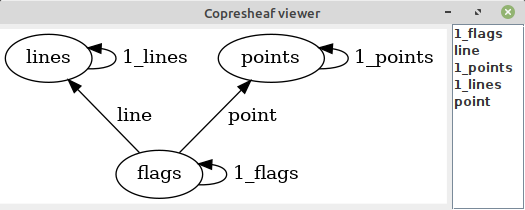
\includegraphics[scale=0.65]{{./incidence.png}}

The objects of this copresheaf topos can often be defined by corresponding set systems, so we will demonstrate a very small part of the set systems library. 

\begin{lstlisting}
; to test for a set system use family of universals
(family-of-universals? #{#{0} #{1})

; a unary family is a set system whose members are all singular
(unary-family? #{#{0} #{1}})

; test for the set theoretic definition of the ordered pair
(kuratowski-pair? #{#{0} #{0 1}})

; check if a set is a power set
(power-set #{#{} #{0} #{1} #{0 1})

; test if the family is subsingleton closed nullfree and rank two
(dependency-family? #{#{0} #{1} #{2} #{0 1} #{1 2}})

; test for open set families of alexandrov topologies
(alexandrov-family? #{#{} #{0} #{0 1} #{0 1 2}})

; test for families of principal ideals of preorders
(preorder-containment-family? #{#{0} #{0 1} #{2} #{2 3}})
\end{lstlisting}

Let $F$ be a family of sets, then we call the members of sets of $F$ dimembers for short. Thus the dimembers function gets all members of the union of a set system. Maximal and minimal dimembers get maximal and minimal elements from preorder containment families, while maximal and minimal members get the sets that are minimal and maximal under inclusion.

\newpage 

In addition to the comprehensive ontology of set systems that we sampled earlier, we also provide a novel and new ontology of multiset systems. A set of multisets is called a clan.

\begin{lstlisting}
(clan? (set (map multiset '((0) (1) (1 1 2))))
\end{lstlisting}

An order pair is a set system like $\{\{0\},\{0, \, 1\}\}$ which combines to form a multiset like $\{0,0,1\}$ or a set system like $\{\{0\}\}$ which combines to form $\{0\}$. Sets of multisets of these forms are called kuratowski clans in our ontology.

\begin{lstlisting}
(kuratowski-clan?
  (set 
    (map 
      multiset 
      '((0) (1) (2) (0 0 1) (0 0 2) (1 1 2)))))
\end{lstlisting}

The set theoretic definition of an ordered pair has to produce different representations based upon repetition, but multisets don't have that problem. A progression clan is the family of initial segments of sequences represented as a multiset, so this forms a general multiset theoretic definition of finite ordered tuples.

\begin{lstlisting}
(progression-clan 0 1 0)
;=> #{*{0} *{0 1} *{0 0 1}}
\end{lstlisting}

Membership in the class of progression clans is then simply checked by the progression-clan? function. At this point, we should mention how we can convert such objects back to the topos $Sets^{[1, \, 2]}$. This is achieved by family->copresheaf and system->copresheaf.

\begin{lstlisting}
; convert a set system into a copresheaf
(family->copresheaf 
  #{#{} #{0} #{0 1} #{0 1 2} #{0 1 2 3}})

; convert a multiset system into a copresheaf
(system->copresheaf 
  (set
    (map
      multiset
      '((0) (1) (2) (0 0 1) (0 0 2)))))
\end{lstlisting}

The objects in the copresheaf topos $Sets^{[1, \, 2]}$ act like multiset systems in general. Therefore, set systems have to be embedded in $Sets^{[1, \, 2]}$ as those for which the point and line functions are together injective and each line has a different set of points associated to it.

\newpage 

\section{Higher order quivers and relations}
There is no reason to think that the basic definition of the topos $Quiv$ cannot be generalized to an index category containing more arrows:

\noindent 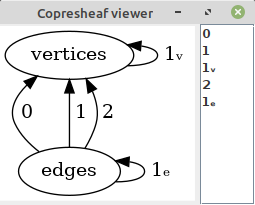
\includegraphics[scale=0.65]{{./ternaryquiver.png}}

This leads to our theory of higher order relations and quivers. A higher order relation is an object of the topos $Sets$ that consists of ordered tuples. While a higher order quiver is a corresponding object in a different copresheaf topos. \\

In order to aid in computations over the topos $Sets$, we provided means for working with a wide variety of relations, including algebraic operations expressed as ternary relations. The following code demonstrates a group represented as a ternary relation.

\begin{lstlisting}
(group-relation? '#{(0 0 0) (0 1 1) (1 0 1) (1 1 0)}) 
\end{lstlisting}

In order to convert that into a corresponding copresheaf, we use the nary-quiver function.

\begin{lstlisting}
; a group represented as an object of the topos Sets^(T2,3)
(nary-quiver '#{(0 0 0) (0 1 1) (1 0 1) (1 1 0)})
\end{lstlisting}

Of course a group is neither a set nor a higher order quiver, but rather an index category for its own topos of GSets. We define the extra representational formats as part of a broader effort to provide support for copresheaves.

\begin{lstlisting}
(quaternary-relation? '#{(0 0 0 0) (1 1 1 1)})
\end{lstlisting}

The nary-quiver is overloaded to work with higher order relations:

\begin{lstlisting}
; a quaternary relation in the topos Sets^(T2,4)
(nary-quiver '#{(0 0 0 0) (1 1 1 1)})
\end{lstlisting}

This copresheaf producing function can be used to create a whole new class of copresheaves to use in our computations. At the same time, a vast ontology of classes of relations is provided as part of our system for supporting the topos $Sets$.

\newpage 

\section{Functional dependencies as copresheaves}
A function is treated as a binary relation with a single functional dependency $\{0\} \to \{1\}$ and this is treated in the topos $Sets$. On the other hand, a bijection is a relation with two functional dependencies $\{0\} \to \{1\}$ and $\{1\} \to \{0\}$ and this leads to a different topos $Sets^{K_2}$. It seems there are different topoi for different types of relations classified by functional dependencies, and so we have special code for handling this correspondence.

\begin{lstlisting}
; create a ternary relation
(def rel 
  '#{(0 0 0) (0 1 1) (1 0 1) (1 1 0)})
  
; compute its set of functional dependencies
(def dep 
  (nary-functional-dependencies rel 3))
\end{lstlisting}

Given a relation and a set of its functional dependencies expressed as a preorder $C$, we can then compute a copresheaf in the topos $Sets^C$.

\begin{lstlisting}
; get a copresheaf on the relation rel
(functional-dependencies-copresheaf rel dep)
\end{lstlisting}

The general set of functional dependencies on a relation can get large and unwieldly at times. In particular, for every relation $R$ the restriction relations $A \to B$ where $B \subseteq A$ are always in the set of dependencies $D$. We may often want to limit ourselves to functional dependencies on individual slots. This for example, can be used to create a trijection in the topos $Sets^{K_3}$.


\begin{lstlisting}
(def trijection 
  '#{(0 1 2) (2 0 1) (1 2 0)})
  
(def dependencies 
  (nary-singleton-functional-dependencies rel 3))
  
(functional-dependencies-copresheaf rel dep)
\end{lstlisting}

Much like the topos of bijections, $Sets^{K_3}$ is basically similar to the topos $Sets$ and so its elements can be created in this way from copresheaves of relations. This is a broad and powerful way that we can create new sources of copresheaves, and it is part of our unification of functional and logical programming. Dependency copresheaves associate relations used in logic programming to the functions most relevant to them. Functional dependency copresheaves are a broad generalisation of topological sheaf theory. Sheaves are limited to consideration of one type of functional dependency: restriction because that is the only type of functional dependency that applies to general classes of functions.

\newpage 

\section{Simplicial methods}
A simplicial set is a copresheaf on the cosimplex category:

\[ f: \Delta^{op} \to Sets \]

A more familiar index category is the simplex category $\Delta$, which is simply the full subcategory of $Cat$ of finite non-empty total orders. But the copresheaves over $\Delta$ are not as interesting as those over $\Delta^{op}$ because they don't have the relevant combinatorial properties, so we are left with defining the cosimplex category by duality.

\[ f : \Delta \to Sets \]

The simplex category and the cosimplex category are both defined as instances of singleton classes: SimplexCategory and CosimplexCategory respectively.

\begin{lstlisting}
; simplex and cosimplex categories have unique instances
simplex-category 
;=> the category of non-empty finite total orders

cosimplex-category 
;=> the dual category of the simplex category

; these two categories override the dual multimethod
(= (dual simplex-category) cosimplex-category)
;=> true

(= (dual cosimplex-category) simplex-category)
;=> true
\end{lstlisting}


These two categories form the dual topoi of simplicial sets $Sets^{\Delta^{op}}$ and of cosimplicial sets $Sets^{\Delta}$. In order to create a simplicial set, use the cosimplex-category as the argument to the Copresheaf constructor in the category field. Unlike the more basic objects of elementary topos theory, simplicial sets cannot be viewed in the copresheaf viewer because the index category $\Delta$ is infinite. \\

Given a copresheaf, the structure-description function will recognise that it is either a simplicial-set or a cosimplex-set based upon the category field value of the Copresheaf instance. Additional functionality include face-morphism? and degeneracy-morphism? for detecting the main types of morphisms in $\Delta$ and face-morphism and degeneracy-morphism which can be used for creating them. A simplicial set can then be created by using the face and degeneracy morphisms as generating sets.

\newpage 

\chapter{Grothendeick topos theory}

\section{Sites}
In order to form elementary topoi, we take start with an index category $C$ and form its copresheaf topos $Sets^C$. On the other hand, to form a Grothendeick topos, we can start with a site $C$ and form its topos of sheaves $Sh(X)$. This requires that we first form a class for dealing with sites. \\ 

The class for sites has only one more field than that for categories: the field for dealing with coverages. A coverage is a function which takes an object $X$ and produces a predicate function which tests for membership in a class of families of morphisms with target at $X$ in the underlying category $C$. We choose to parameterize coverages by objects.

\begin{lstlisting}
; one of the most basic types of site
(discrete-site #{0 1 2 3})

; the dual notion of a discrete site
(indiscrete-site #{0 1 2 3})

; create a topological site on the Sierpinski space
(topological-site #{#{} #{0} #{0 1}})

; create a topological site on four points
(topological-site #{#{} #{0} #{0 1} #{0 2} #{0 1 2} #{0 1 2 3}})
\end{lstlisting}

You can also create a Site by using the adjoin-coverage function to add a coverage to an existing category. We now use the predicates site? and elementary-category? to refer to the two different types of category that come out of site theory. As the category of copresheaves associated to categories that aren't sites are called elementary topoi, we call every category that isn't a site an elementary category. So that site? and elementary-category? are complements of one another in the universe of categories.

\newpage 

The predicates elementary-category and site? are demonstrated below:

\begin{lstlisting}
(elementary-category? (n-arrow-category 2))
;=> true

(site? (n-arrow-category 2))
;=> false

(elementary-category? (discrete-site #{0 1 2}))
;=> false 

(site? (discrete-site #{0 1 2}))
;=> true
\end{lstlisting}

We can also create a site by adjoining a coverage function to an existing category.

\begin{lstlisting}
; convert an existing category into a site
(adjoin-coverage category func)
\end{lstlisting}

In the other direction, to convert a site back into an elementary category use the to-category method.

\begin{lstlisting}
; convert a site into an elementary category 
(to-category site)
\end{lstlisting}

Here is how you can get the family of morphism systems that cover an object of a site:

\begin{lstlisting}
; get all coverings of an object of a site
(let [cov (.-coverage site)]
  (cov obj))
\end{lstlisting}

Grothendeick sites play the role that elementary categories do in elementary topos theory, but for Grothendeick topoi. In that case, the objects of Grothendeick topoi are sheaves on a site.

\section{Sheaves}
Let $C$ be a site then a sheaf on $C$ is a presheaf on the site that satisfies the covering condition, thusly in order to convert it into a copresheaf you can define it in terms of the dual category $C^{op}$. So naturally one way to create a sheaf would be to define a copresheaf on $C^{op}$ so that sheaves can be integrated into our copresheaf paradigm. A sheaf could also be defined as a special class of objects with a computable gluing function, especially when they are defined over topological spaces.

\newpage 

\chapter{Topos theory of structure}

\section{Multi-sorted structures}
Topos theory can easily be extended to deal with multi-sorted structures containing collections of sets. The key is to define a functor to a topos $Sets^n$ of collections of sets. An example is the category of graphs, which can be described in terms of the topos $Sets^2$. \\

\noindent 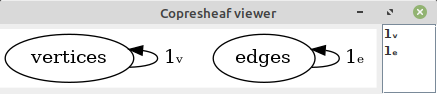
\includegraphics[scale=0.65]{{./graph.png}}

A graph is defined as an ordered pair $(V,E)$ and a morphism of graphs is a function $f: (V,E) \to (V',E')$ such that $\forall {a,b} \in E : {f(a),f(b)} \in E$. Then we define a morphism to $Sets^2$ that maps $(V,E)$ to $(V,E)$ and that maps $f : (V,E) \to (V',E')$ to the pair of functions $(g : V \to V', h: E \to E')$ with $g$ defined by the underlying function of $f$ and $h$ defined by the image functor restriction $E$ $\wp(f)_E$. It follows that $m : Graph \to Sets^2$ is a functor.

\begin{lstlisting}
; create an instance of the graph class
(def g (Graph. #{0 1 2} #{#{0} #{1} #{2} #{0 1} #{1 2}}))

; convert it into an object in the topos of disets
(to-copresheaf g)
\end{lstlisting}

The same basic process used here can be applied to digraphs, hypergraphs, or any other graph like structures consisting of vertices and edges. In each case their copresheaf form can be computed by the to-copresheaf function which produces a copresheaf in the topos $Sets^2$. This occurs because graphs and hypegraphs are defined as multi-sorted structures defined by collections of sets, however, we can also define incidence functors in the topos $Sets^{[1, \, 2]}$ from them. 
 
\newpage 

Incidence structures are multi-sorted structures that are built out of three sets, and so they naturally form functors to the topos of trisets $Sets^3$.
\\ \\
Definition. an incidence structure is an ordered triple $(V,E,F)$ with $F \subseteq V \times E$ and a morphism of incidence structures $m: (V,E,F) \to (V',E',F')$ is a pair of maps $f: V \to V'$ and $g : E \to E'$ such that for each $(a,b) \in F$ we have that $(f(a),g(b)) \in F'$.
\\ \\
Then we define a functor to $Sets^3$ that maps $(V,E,F)$ to $(V,E,F)$ and $m: (V,E,F) \to (V',E',F')$ by the triple of functions $(f,g,f \times g)$ which is a morphism in the topos $Sets^3$. \\

\noindent 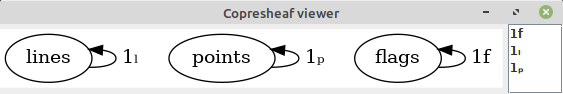
\includegraphics[scale=0.65]{{./incidencetriple.png}}

The definition of this functor leads to our implementation of incidence structures as copresheaf objects of the topos $Sets^3$.

\begin{lstlisting}
; create an inccidence structure from a graph
(def incidence-structure
  (to-incidence-structure 
    (family->hypergraph #{#{0} #{0 1} #{0 1 2}})))

; convert the incidence structure into a copresheaf
(to-copresheaf incidence-structure)
\end{lstlisting}

As an incidence structure can be understood either by the topos $Sets^3$ or by the topos $Sets^{[1,\,2]}$ we have a separate function for creating a different type of copresheaf from incidence structure objects:

\begin{lstlisting}
(to-span-copresheaf incidence-structure)
\end{lstlisting}

The matrix module also contains means for converting incidince structures like these into matrices. Use the to-incidence-matrix function to get a matrix from an incidence structure. The same function can be applied to graphs or hypergraphs, as it is an overloaded multimethod. \\ 

A number of functions are provided specifically for incidence structures. The dual incidence structure creates the dual structure defined by swapping points and lines. It corresponds to the transpose of the incidence matrix. The complement-incidence-stucture function produces the complement of $(V,E,F)$ which is $(V,E,V\times E - F)$. Membership testing for the class of incidence structures is implemented by the incidence-structure? predicate.

\newpage 

\section{Topos theoretic foundations of algebra}
In universal algebra we define a n-ary operation on $S$ to be a function with the signature $f: S^n \to S$. We then say that $m : S \to T$ is a morphism of n-ary operations $f : S^n \to S$ and $T^n \to T$ provided that $m(f(a,b,c,...)) = g(m^n(a,b,c,..))$. This leads to a commutative diagram:

\noindent 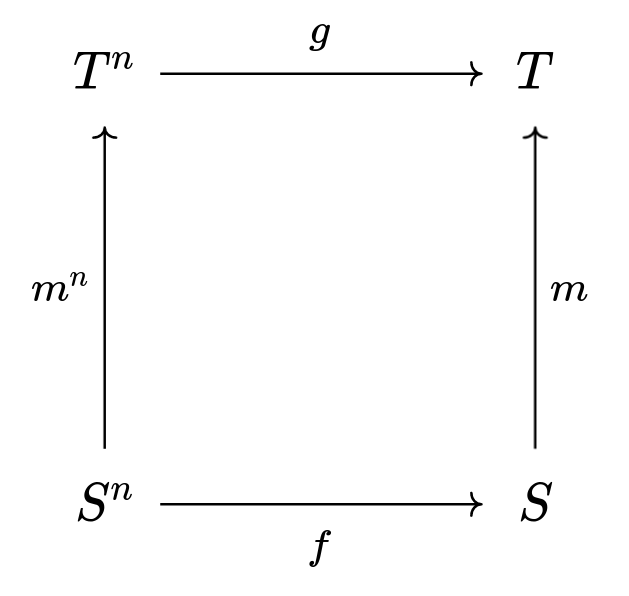
\includegraphics[scale=0.25]{{./commutativediagram.png}}

Which means that $(m^n,m)$ is a morphism of functions from $f$ to $g$, and this generalises to n-ary operations of any size. An algebra can be defined by a set $S$ with a set of different functions $f_i : S^n \to S$. The class of all algebras with a given indexed collection of functions $f_i : S^n \to S$ over an index set $I$ with a given signature forms a category $Alg$ of algebras. \\

Each of these indices determines a functor to the topos $Sets^{\to}$ that maps an algebra $A$ to its $i$ indexed function, and that maps a morphism of algebras to its corresponding morphism of functions determined in the commutative diagram above. 

\[ F_i : Alg \to Sets^{\to} \]

Let $A$ be an algebra and let $c$ be a congruence of it. Then this morphism $F_i$ induces a congruence for each $i$ indexed function of arity $i$ by the ordered pair of equivalence relations $(C^2,C)$ which is a congruence in the topos $Sets^{\to}$. This implies that a congruence in universal algebra is simply a way of describing part of the computational logic of data dependencies. \\

These functors are therefore important in our burgeoning theory of congruences of the topos $Sets^{\to}$. By making use of the topos $Sets^{\to}$ in order to do universal algebra, we can finally put abstract algebra on a good solid foundation based upon topos theory. The dual logic is defined by the mapping over subalgebras which takes any subalgebra $S \subseteq A$ and maps an nary operation to the subobject $(S^n,S)$ in the topos $Sets^{\to}$. Together with the epi-mono factorisation inherent in any topos, we have a factorisation in terms of $(C^n,C)$ and $(S^n,S)$ which generalises the homomorphism theorems.

\newpage 

An algebra is defined by a collection of functions that have the same target, so we can use a cospan copresheaf to represent algebras. A ring $(R,+,*,-,0,1)$ is depicted as a copresheaf below: \\

\noindent 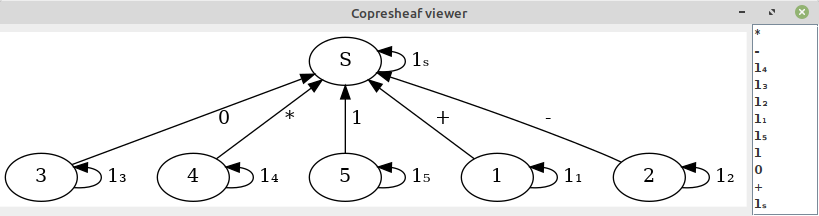
\includegraphics[scale=0.5]{{./ring.png}}

This same process is applicable to any number of different constructs in universal algebra constructed by sets of function symbols, and by considering things in terms of copresheaves we get the best possible foundations. A number of functions are built in for creating rings.

\begin{lstlisting}
; create a ring in terms of its tables
(def gf3
  (make-ring 
    (group-by-table 
      [[0, 1, 2]
       [1, 2, 0]
       [2, 0, 1]])
    (monoid-by-table
      [[0, 0, 0]
       [0, 1, 2]
       [0, 2, 1]])))
       
; convert the ring into a copresheaf
(to-copresheaf ring)
\end{lstlisting}

The sub and con methods are overriden for dealing with rings. The subalgebra lattice computation using Lagrange's theorem and the congruence lattice computation uses ideals.

\begin{lstlisting}
; compute the subalgebra lattice of a ring
(sub gf3)

; compute the congruence lattice of a ring 
(con gf3)
\end{lstlisting}

Given any normal subgroup we can convert it into a congruence by its left or right cosets. In the case of an ideal we can get a congruence by applying this to its additive group.

\newpage

Support is also provided for semirings, by generalisation of rings, some of the most interesting are those that come from other structures. 

\begin{lstlisting}
; the semiring of ideals of a ring
(semiring-of-ideals gf3)

; get the semiring of morphism systems of a category
(semiring-of-morphism-systems (n-arrow-category 2))
\end{lstlisting}

In addition, we provide support for semimodules and modules. We can convert commutative monoids into $\mathbb{N}$ semimodules and commutative groups into $\mathbb{Z}$ modules.

\begin{lstlisting}
(to-semimodule (monogenic-monoid 4 1))
(to-module (cyclic-group 3))
\end{lstlisting}

We also provide support for generic operations over semirings using Clojure's builtin symbols +,*,-,/ but redefined to handle overloaded arithmetic.

\begin{lstlisting}
(def m (binary-matrix [[0,0],[1,0]]))
(def n (binary-matrix [[0,1],[0,0]]))

(+ m n)
;=> [[0,1],[1,0]]

(* m n)
;=> [[0,0],[0,1]]
\end{lstlisting}

A number of classes of arithmetic objects like rational functions, polynomials, and power series are already supported. Furthermore, we provide general support for semigroup algebras over rings and semirings.

\begin{lstlisting}
; ring of laurent polynomials over the integers
(semigroup-algebra zz (free-commutative-group #{0 1 2}))

; polynomial semiring on three variables
(semigroup-algebra nn (free-commutative-monoid #{0 1 2}))

; semigroup semiring of set systems on three elements
(semigroup-algebra t2 (free-semilattice #{0 1 2}))
\end{lstlisting}

With the theory of semigroup semirings we can establish additional structures on the set of multiset systems or multirelations on a set. These interpret multirelations and multiset systems as semigroup semirings of the natural numbers over the non-commutative free monoid and the commutative free monoid respectively. The arithmetic operations of these two semigroup semirings are provided by the multiply-multirelations and multiply-multiclan functions.

\newpage

\chapter{Ontology}

\section{Classification of copresheaves}
As our system is constructed entirely around a bunch of different types of copresheaves, it remains to add some structure to all this copresheaf theory. Below is a diagram representing the different types of copresheaves and their inclusions. \\ \\

\noindent 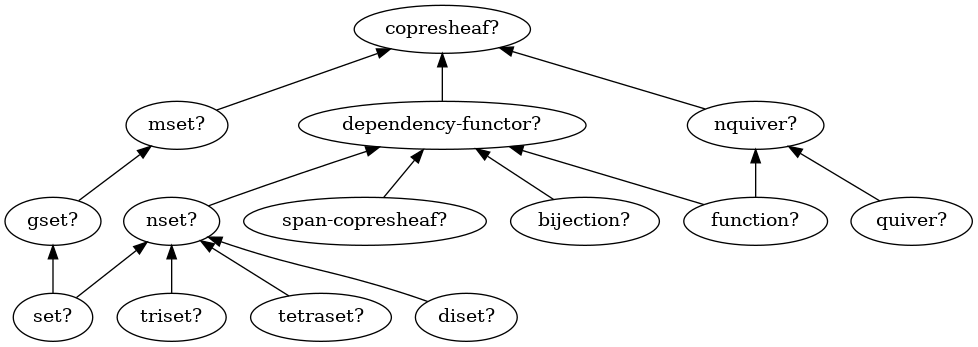
\includegraphics[scale=0.4]{{./ontology.png}} \\

We will construct our entire mathematical ontology around copresheaves over various categories. The first stage is described here by classifying copresheaves based upon their categorical properties, like the structure of their index categories. The next step would then be to describe particularities of various different types of copresheaves. For example, the set ontology might diverge into a wide range of different sets like relations, families of sets, sets of functions, etc. The function ontology might diverge into binary operations, set valued functions, etc. Quivers can be classified by their graph theoretic properties, and so on. Finally, a later version of this program may be extended to include schemes and sheafs of rings.

\chapter{Interfaces}

\section{Apache commons math}
The apache commons math library provides a number of pieces of functionality that we do not care to implement ourselves, and so we should use it as much as possible. As long as the apache commons math system keeps its basic focus on numerical analysis, statistics, probability, computational geometry, etc there shouldn't be much overlap with it.

\begin{lstlisting}
; create a complex number using apache commons math
(def num (complex-number 1 2))

; perform arithmetic on it using overloaded operations
(+ num num)
(* num num)

; create a quaternion using apache commons math
(def quaternion-number (quaternion 1 2 3 4))

; complex numbers and quaternions using our ring datatype
quaternions
complex-numbers
\end{lstlisting}

We also provide support for FieldMatrices and interfaces to the linear package, but we provide our own SemiringMatrix class simply because the apache commons math library doesn't handle semirings. \\ 

Other libraries we may use in the future include JFreeChart, sat4j, the choco solver, renjin, JGraphT or some other graph library, etc. We may also use the Java language for some classes. This should make it easier to integrate this project into existing programs that use other JVM libraries. We will continue to make enthusiastic use of the JVM because it is the best platform for the free choice of languages like Clojure.

\end{document}
